\documentclass[11pt]{iopart}
\usepackage[english]{babel}
\pdfoutput=1
%\usepackage{amsmath}
\usepackage{wasysym}
\usepackage{booktabs}
\usepackage{amssymb}
\usepackage{amsbsy}
\usepackage{verbatim}
\usepackage{graphicx}
\usepackage{epstopdf}
\usepackage{color}
\usepackage{sidecap}
\usepackage{bm}% bold math
\usepackage{tikz}
%\usepackage[backend=bibtex]{biblatex}

\usepackage[colorlinks,bookmarks=false,citecolor=blue,linkcolor=red,urlcolor=blue]{hyperref}

\newcommand*\circled[1]{\tikz[baseline=(char.base)]{
            \node[shape=circle,draw,inner sep=2pt] (char) {#1};}}


%\usepackage{cite}

%
% WARNING !!!!
% 
% iopart.cls definition of \tableofcontents overwrites the
% short title printed every page. 
% The following redefinition of \tableofcontents fixes the
% the problem. 

\catcode`@=11 % If we need private TeX macros
\renewcommand\tableofcontents{%
  \section*{\contentsname}%
  \@starttoc{toc}%
}
\catcode`@=12% '@' is no more a character
\newcommand{\bra}[1]{\langle\left.{#1}\right|}
\newcommand{\ket}[1]{\left|{#1}\right.\rangle}


\def\be{\begin{equation}}
\def\ee{\end{equation}}
\def\u{\uparrow}
\def\d{\downarrow}
\def\nm{\newmoon}
\def\fm{\fullmoon}
\def\T{\rule{0pt}{.6cm}}
\def\B{\rule[-.4cm]{0pt}{0pt}}

\begin{document}

\setlength{\parindent}{0pt}


\title{The quench action approach for integrable models: A Monte Carlo implementation}

\author{Authors}
%\address{$^1$ International School for Advanced Studies (SISSA),
%Via Bonomea 265, 34136, Trieste, Italy,
%INFN, Sezione di Trieste}


\date{\today}



%%%%%%%%%%%%%%%%%%%%%%%%%%%%%%%%%%%%%%%%%%%%%%%%%%%%%%%%%%%%%%%%%%%%%%%%%%
\begin{abstract} 


fdasfa
\end{abstract}

\maketitle

%%%%%%%%%%%%%%%%% INTRODUCTION %%%%%%%%%%%%%%%%%%%%%
\section{Introduction}
\label{intro}

We show that it is possible to numerically simulate the Quench Action approach 
combining Monte Carlo methods and Bethe ansatz techniques. 

We focus on the situation in which the pre-quench initial state is the Neel 
state or the Majumdar-Ghosh state. 

We investigate the importance of the zero-momentum strings in the Quench Action. 

Without zero-momentum strings the overlap saturation rules are not valid, 
i.e., in finite size systems the vast majority of the eigenstates contain 
zero momentum strings. 

The details on the eigenstates counting depend on the pre-quench initial state. 

However, we show that one can restrict to the set of non-zero momentum strings. 
The fact that one neglects zero-momentum strings gives rise only to scaling 
corrections. 

We also investigate the validity of the Bethe-Takahashi approximation for the 
calculation of the overlap. 

In the thermodynamic limit it is natural to assume that the steady-state expectation 
values are obtained using the so-called diagonal ensemble, which is defined as 
%
\begin{equation}
\label{d-ensemble}
\langle{\mathcal O}\rangle=\sum\limits_{\alpha}|\langle\Psi_0|\alpha\rangle|^2
\langle\alpha|{\mathcal O}|\alpha\rangle. 
\end{equation}
%

It is useful to rewrite~\eref{d-ensemble} as 
%
\begin{equation}
\label{qa-prob}
\langle{\mathcal O}\rangle=\sum\limits_{\alpha}\rho^{DE}(\alpha)
\langle\alpha|{\mathcal O}|\alpha\rangle,\quad\textrm{with}\quad 
\rho^{DE}(\alpha)=\exp(-2\Re{\mathcal E}(\alpha)).
\end{equation}
%
Here $\rho^{DE}(\alpha)$ is a diagonal ensemble density matrix, and ${\mathcal E}(\alpha)
\equiv-\log\langle\alpha|\Psi_0\rangle$, with $\Re$ denoting the real part. 

%%%%%%%%%%%%%%%%%%%%%%% BETHE ANSATZ FOR THE XXX CHAIN %%%%%%%%%%%%%%%%%%%%%%%%%%
\section{Bethe ansatz solution of the Heisenberg ($XXX$) spin chain}
\label{sec:1}

Here we review some Bethe ansatz results for the spin-$\frac{1}{2}$ Heisenberg 
($XXX$) chain. Specifically, in section~\ref{sec:1.1} we introduce the model. 
Its eigenstates (Bethe states) and the Bethe equations are discussed in 
section~\ref{sec:1.2}. Section~\ref{sec:1.3} focuses on the string hypothesis 
and the so-called Bethe-Gaudin-Takahashi (BGT) equations. The form of the 
BGT equations in the thermodynamic limit is discussed in section~\ref{sec:1.4}. 
Finally, in section~\ref{sec:1.5} we provide some exact formulas for the 
local conserved charges of the model. 


%%%%%%%%%%%%%%%%%%%%%%%%%%%%%%%%%%%%%%%%%%%%%%%%%%%%%%%%%%%%%%%%%%%%%%%%%%%
\subsection{The spin-$\frac{1}{2}$ Heisenberg chain}
\label{sec:1.1}

The spin-$\frac{1}{2}$ isotropic Heisenberg chain ($XXX$ chain) with $L$ sites 
is defined by the Hamiltonian 
%
\begin{equation}
\label{xxx-ham}
{\mathcal H}\equiv J\sum\limits_{i=1}^L\left[\frac{1}{2}(S_i^+S^-_{i+1} 
+S_i^{-}S_{i+1}^+)+S_i^zS_{i+1}^z-\frac{1}{4}\right],  
\end{equation}
%
where $S^{\pm}_i\equiv (\sigma_i^x\pm i\sigma_i^y)/2$ are spin operators acting on the 
site $i$, $S_i^z\equiv\sigma_i^z/2$, and $\sigma^{x,y,z}_i$ the Pauli matrices. We fix 
$J=1$ and use periodic boundary conditions, identifying sites $L+1$ and $1$. The total 
magnetization $S_{T}^z\equiv\sum_iS_i^z=L/2-M$, with $M$ number of down spins (particles), 
commutes with~\eref{xxx-ham}, and it is here used to label its eigenstates. 


%%%%%%%%%%%%%%%%%%%%%%%%%%%%%%%%%%%%%%%%%%%%%%%%%%%%%%%%%%%%%%%%%%%%%%%%%%%
\subsection{Bethe equations and wavefunctions}
\label{sec:1.2}


In the Bethe ansatz framework~\cite{bethe-1931,taka-book} the generic eigenstate 
of~\eref{xxx-ham} (Bethe state) in the sector with $M$ particles can be written as 
%
\begin{equation}
\label{ba-eig}
|\Psi_M\rangle=\sum\limits_{1\le x_1<x_2<\dots<x_M\le L}A_M(x_1,x_2,
\dots,x_M)|x_1,x_2,\dots,x_M\rangle,
\end{equation}
%
where the sum is over the positions $\{x_i\}_{i=1}^M$ of the particles, and $A_M(x_1,
x_2,\dots,x_M)$ is the eigenstate amplitude corresponding to the particles 
being at positions $x_1,x_2,\dots, x_M$. Here $A_M(x_1,x_2,\dots, x_M)$ is 
given as 
%
\begin{equation}
\label{ba_amp}
A_M(x_1,x_2,\dots,x_M)\equiv\sum\limits_{\sigma\in S_M}\exp\Big[i
\sum\limits_{j=1}^Mk_{\sigma_j}x_j+i\sum\limits_{i<j}\theta_{\sigma_i,\sigma_j}
\Big], 
\end{equation}
%
where the outermost summation is over the permutations $S_M$ of the so-called 
quasi-momenta $\{k_\alpha\}_{\alpha=1}^M$. The two-particle scattering phases 
$\theta_{\alpha,\beta}$ are defined as 
%
\begin{equation}
\label{s_phases}
\theta_{\alpha,\beta}\equiv \frac{1}{2i}\log\Big[-\frac{e^{ik_\alpha+ik_\beta}-
2e^{ik_\alpha}+1}{e^{ik_\alpha+ik_\beta}-2e^{ik_\beta}+1}\Big].
\end{equation}
%
The eigenenergy associated to the eigenstate~\eref{ba-eig} is  
%
\begin{equation}
\label{ba-ener}
E=\sum\limits_{\alpha=1}^M(\cos(k_\alpha)-1). 
\end{equation}
%
The quasi-momenta $k_\alpha$ are obtained by solving the so-called Bethe 
equations~\cite{bethe-1931}
%
\begin{equation}
\label{ba-eq}
e^{ik_\alpha L}=\prod\limits^M_{\beta\ne\alpha}\Big[-\frac{1-2e^{
ik_\alpha}-e^{ik_\alpha+ik_\beta}}{1-2e^{ik_\beta}-e^{ik_\alpha+
ik_\beta}}\Big].
\end{equation}
%
It is useful to  introduce the rapidities $\{\lambda_\alpha\}_{\alpha=1}^M$ as 
%
\begin{equation}
\label{rap}
k_\alpha=\pi-2\arctan(\lambda_\alpha)\quad\mbox{mod}\, 2\pi.
\end{equation}
%
Taking the logarithm on both sides in~\eref{ba-eq}, and using~\eref{rap}, 
one obtains the Bethe equations in logarithmic form as 
%
\begin{equation}
\label{ba-eq-log}
\arctan(\lambda_\alpha)=\frac{\pi}{L}J_\alpha+\frac{1}{L}\sum\limits_{
\beta\ne\alpha}\arctan\Big(\frac{\lambda_\alpha-\lambda_\beta}{2}\Big),
\end{equation}
%
where $-L/2<J_\alpha\le L/2$ are the so-called Bethe quantum numbers. The 
$J_\alpha$ are half-integers and integers for $L-M$ even and odd, 
respectively. 

Finally, one should remark that $M$-particle eigenstates corresponding to 
{\it finite} rapidities are eigenstates with maximum allowed magnetization 
(highest-weight eigenstates) $S_T^z=L/2-M=S_T$, with $S_T$ the total spin. 
Due to the $SU(2)$ invariance of~\eref{xxx-ham}, all the states in the same 
$S_T$ multiplet and different $-S_T\le S_T^z\le S_T$ are eigenstates of the 
$XXX$ chain with the same energy eigenvalue. These eigenstates (descendants) 
are obtained by multiple applications of the total-spin lowering operator 
$S_T^-\equiv\sum_iS_i^-$ on the highest-weight eigenstates. In the Bethe ansatz 
framework the rapidities of a generic $M$-particle descendant eigenstate with 
$S_T^T=L/2-M'$, with $M'<M$, are obtained by supplementing the $M$ rapidities 
of the highest-weight state with $M'-M$  infinite rapidities. We anticipate 
that descendant eigenstates have non-zero overlap with the zero-momentum 
N\'eel state (cf. section~\ref{sec:2}). 
 

%%%%%%%%%%%%%%%%%%%%%%%%%%%%%%%%%%%%%%%%%%%%%%%%%%%%%%%%%%%%%%%%%%%%%%%%%%%
\subsection{String hypothesis \& the Bethe-Gaudin-Takahashi (BGT) equations}
\label{sec:1.3}

In the thermodynamic limit $L\to\infty$ the solutions of the Bethe 
equations~\eref{ba-eq} form particular ``string'' patterns in the complex plane, 
(string hypothesis)~\cite{bethe-1931,taka-book}. Specifically, the rapidities 
forming a ``string'' of length $1\le n\le M$ (that we defined here as 
$n$-string) can be parametrized as 
%
\begin{equation}
\label{str-hyp}
\lambda^{j}_{n;\gamma}=\lambda_{n;\gamma}-i(n-1-2j)+i\delta_{n;\gamma}^j,\qquad 
j=0,1,\dots, n-1, 
\end{equation}
%
with $\lambda_{n;\gamma}$ being the real part of the string (string center), 
$\gamma$ labelling strings with different centers, and $j$ labelling the different 
components of the string. In Eq.~\eref{str-hyp} $\delta_{n;\gamma}^j$ are the string 
deviations, which typically, i.e., for most of the chain eigenstates, vanish 
exponentially with $L$ in the thermodynamic limit. 
Note that real rapidities correspond to strings of unit length ($1$-strings), i.e., 
$n=1$ in Eq.~\eref{str-hyp}. 


The string centers $\lambda_{n;\gamma}$ are obtained by solving the so-called 
Bethe-Gaudin-Takahashi equations
%
\begin{equation}
\label{bgt-eq}
2L\theta_n(\lambda_{n;\gamma})=2\pi I_{n;\gamma}+\sum\limits_{(m,
\beta)\ne(n,\gamma)}\Theta_{m,n}(\lambda_{n;\gamma}-\lambda_{m;\beta}).  
\end{equation}
%
The generalized scattering phases $\Theta_{m,n}$ read 
%
\begin{eqnarray}
\label{Theta}
\nonumber\fl\Theta_{m,n}(x)\equiv\left\{\begin{array}{cc}
\theta_{|n-m|}(x)+\!\!\!\!\!\sum
\limits_{r=1}^{(n+m-|n-m|-1)/2}\!\!\!\!\!2\theta_{|n-m|+2r}(x)
+\theta_{n+m}(x) & \quad\mbox{if}
\quad n\ne m\\\fl\sum\limits_{r=1}^{n-1}2\theta_{2r}(x)+
\theta_{2n}(x) & \quad\mbox{if}\quad n=m
\end{array}\right.
\end{eqnarray}
%
with $\theta_\alpha(x)\equiv 2\arctan(x/\alpha)$. Here $I_{n;\gamma}$ are the 
Bethe-Takahashi quantum numbers associated with $\lambda_{n;\gamma}$. 
The solutions of~\eref{bgt-eq}, and the Bethe states thereof, are naturally 
classified according to their ``string content'' ${\mathcal S}\equiv\{s_n
\}_{n=1}^M$, with $s_n$ the number of $n$-strings. Clearly, the constraint 
$\sum_{n=1}^{M}n s_n=M$ has to be satisfied. It can be shown that 
the BGT quantum numbers $I_{n;\gamma}$ associated with the $n$-strings are 
integers and half-integers for $L-s_n$ odd and even, respectively. 
An upper bound for the BGT quantum numbers can be derived as~\cite{taka-book} 
%
\begin{equation}
|I_{n;\gamma}|\le I^{(MAX)}_{n}\equiv\frac{1}{2}(L-1-\sum
\limits_{m=1}^Mt_{m,n}s_m),
\label{bt-qn-bound}
\end{equation}
%
where $t_{m,n}\equiv 2\mbox{min}(n,m)-\delta_{m,n}$. Using the string hypothesis 
Bethe states energy eigenvalue~\eref{ba-ener} becomes
%
\begin{equation}
\label{ener-str}
E=-\sum_{n,\gamma}\frac{2n}{\lambda_{n;\gamma}^2+n^2}. 
\end{equation}
%

%%%%%%%%%%%%%%%%%%%%%%%%%%%%%%%%%%%%%%%%%%%%%%%%%%%%%%%%%%%%%%%%%%%%%%%%%%%
\subsection{Thermodynamic limit}
\label{sec:1.4}

In the thermodynamic limit $L\to\infty$ at fixed finite particle density $M/L$ 
the solutions of the BGT equations~\eref{bgt-eq} become dense. One then defines 
the BGT root distributions for the $n$-strings as $\pmb{\rho}\equiv\{\rho_n(
\lambda)\}_{n=1}^\infty$, with $\rho_n(\lambda)\equiv\lim_{L\to\infty}[
\lambda_{n;\gamma+1}-\lambda_{n;\gamma}]^{-1}$. Thus the  BGT 
equations~\eref{bgt-eq} become an infinite set of coupled non-linear integral 
equations for the $\rho_n(\lambda)$ as 
%
\begin{equation}
\label{bgt-th}
a_n(\lambda)=\rho_n(\lambda)+\rho^h_n(\lambda)+\sum_m(T_{n,m}*\rho_m)
(\lambda),
\end{equation}
%
where $\rho_n^{h}$ are the hole-distributions, and the functions $a_n(\lambda)$ 
are defined as 
%
\begin{equation}
a_n(x)\equiv\frac{1}{\pi}\frac{n}{x^2+n^2}. 
\end{equation}
%
In~\eref{bgt-th} $T_{n,m}*\rho_m$ denotes the convolution 
%
\begin{equation}
(T_{n,m}*\rho_m)(\lambda)\equiv\int_{-\infty}^{+\infty}T_{n,m}(\lambda-\lambda')
\rho_{m}(\lambda'),
\end{equation}
%
with the matrix $T_{n,m}(x)\equiv\Theta'(x)$ being dfined as 
%
\begin{eqnarray}
\nonumber\fl T_{m,n}(x)\equiv\left\{\begin{array}{cc}
a_{|n-m|}(x)+\!\!\!\!\!\sum
\limits_{r=1}^{(n+m-|n-m|-1)/2}\!\!\!\!\!2a_{|n-m|+2r}(x)
+a_{n+m}(x) & \quad\mbox{if}
\quad n\ne m\\\fl\sum\limits_{r=1}^{n-1}2a_{2r}(x)+
a_{2n}(x) & \quad\mbox{if}\quad n=m
\end{array}\right.
\end{eqnarray}
%
For a generic smooth enough observable ${\mathcal O}$ in the thermodynamic 
limtit its expectation value is expected to become a functional of the root 
densities $\pmb{\rho}$ as $\langle\pmb{\rho}|{\mathcal O}|\pmb{\rho}\rangle$. 

Moreover, for all the local observables considered in this work the contribution of the 
different type of strings factorize and one can write 
%
\begin{equation}
\langle\pmb{\rho}|{\mathcal O}|\pmb{\rho}\rangle=\sum_{n=1}^\infty
\int_{-\infty}^{+\infty}d\lambda \rho_n(\lambda) {\mathcal O}_n(\lambda), 
\end{equation}
% 
with ${\mathcal O}_n(\lambda)$ the ... .

%%%%%%%%%%%%%%%%%%%%%%%%%%%%%%%%%%%%%%%%%%%%%%%%%%%%%%%%%%%%%%%%%%%%%%%%%%%
\subsection{The conserved charges}
\label{sec:1.5}

The $XXX$ chain exhibits an extensive number of mutually commuting local conserved 
charges $Q_n$, with $n\in\mathbb{N}$, i.e., 
%
\begin{equation}
[Q_n,{\mathcal H}]=0\quad\forall n\quad\textrm{and}\quad [Q_n,Q_m]=0\quad\forall n,m.
\end{equation}
%
The eigenvalues $q_n$ of the conserved charges over the Bethe eigenstates 
(cf.~\eref{ba-eig}) are given as 
%
\begin{equation}
\label{Q-def}
\left.q_{n+1}\equiv\frac{i}{(n-1)!}\frac{d^n}{dy^n}\log\tau
(y)\right|_{y=i},
\end{equation}
%
where $y$ is a spectral parameter and $\tau(y)$ is the Bethe state eigenvalue of the 
so-called transfer matrix in the Algebraic Bethe Ansatz framework~\cite{kor-book}. 
The analytic expression for $\tau(y)$ in terms of the solutions 
$\{\lambda_\alpha\}_{\alpha=1}^M$ of the Bethe equations~\eref{ba-eq} is given as 
%
\begin{equation}
\label{tau}
\tau(y)\equiv\Big(\frac{y+i}{2}\Big)^L\prod\limits_\alpha\frac{y-\lambda_\alpha-2i}
{y-\lambda_\alpha}+\Big(\frac{y-i}{2}\Big)^L\prod\limits_\alpha\frac{y-\lambda_\alpha
+2i}{y-\lambda_\alpha}.
\end{equation}
%
Interestingly, from~\eref{Q-def} one has that the second term in~\eref{tau} does not 
contribute to $q_n$, at least for $n\le L-2$. 
For a generic Bethe state $q_n$ is obtained by summing independently the contributions 
of the BGT roots as 
%
\begin{equation}
\label{qngnk}
q_n=\sum_{k,\gamma}g_{n,k}(\lambda_{k;\gamma}).
\end{equation}
%
Using the string hypothesis~\eref{str-hyp}, and~\eref{Q-def},~\eref{tau}, one obtains  
the the first few functions $g_{n,k}$ in terms of the solutions of the BGT equations as 
%
\begin{eqnarray}
\label{gnk}
g_{3,k}=-\frac{4k\lambda_{k;\gamma}}{(\lambda_{k;\gamma}^2+k^2)^2}, &\quad  
g_{4,k}=\frac{2k(k^2-3\lambda_{k;\gamma}^2)}{(k^2+\lambda_{k;\gamma}^2)^3}\\\nonumber 
g_{5,k}=\frac{8k\lambda_{k;\gamma}(k^2-\lambda_{k;\gamma}^2)}{(k^2+
\lambda_{k;\gamma}^2)^4}, & \quad
g_{6,k}=-\frac{2k(5\lambda_{k;\gamma}^4-10k^2\lambda_{k;\gamma}^2+k^4)}{(k^2+
\lambda_{k;\gamma}^2)^5}. 
\end{eqnarray}
%
Note that $q_2$ is the Bethe state energy eigenvalue and is given in~\eref{ener-str}. 
It is also interesting to observe that $g_{n,k}$ (cf.~\eref{gnk}) is vanishing for 
infinite BGT roots. This is expected to hold for the generic $g_{n,k}$, i.e., for any 
$n$, and it is a consequence of the $SU(2)$ invariance of the conserved charges. Finally, 
in the thermodynamic limit $L\to\infty$ from~\eref{qngnk} one has 
%
\begin{equation}
\label{q0-th}
q_n\to\sum_{k=1}^\infty\int_{-\infty}^{+\infty}d\lambda\rho_k(\lambda)g_{n,k}(\lambda), 
\end{equation}
%
where the BGT root distributions $\rho_k(\lambda)$ are solutions of~\eref{bgt-th}. 



%%%%%%%%%%%%%%%%%%%%%%%%%%%%%%%%%%%%%%%%%%%%%%%%%%%%%%%%%%%%%%%%%%%%%%%%%%%
\section{Overlap between the Bethe states and some initial states} 
\label{sec:2}

%%%%%%%%%%%%%%%%%%%%%%%%%%%%%%%%%%%%%%%%%%%%%%%%%%%%%%%%%%%%%%%%%%%%%%%%%%%
\subsection{N\'eel state overlap}

Here we detail the Bethe ansatz results for the overlap of the Bethe states (cf.~\eref{ba-eig}) 
with the zero-momentum (one-site shift invariant) N\'eel state $|N\rangle$ and the 
Majumdar-Ghosh (MG) $|MG\rangle$ state. We stard discussing the N\'eel state. This is 
defined as 
%
\begin{equation}
\label{neel}
|N\rangle\equiv\frac{1}{\sqrt{2}}\big(|N_1\rangle
+|N_2\rangle\big), 
\end{equation}
%
with $|N_1\rangle\equiv |\uparrow\downarrow\rangle^{\otimes L/2}$, and $|N_2\rangle\equiv 
|\downarrow\uparrow\rangle^{\otimes L/2}$. Note that $|N_1\rangle=\hat T|N_2\rangle$, 
with $\hat T$ the one-site shift operator. 

Due to the zero-momentum constraint, only parity-invariant Bethe states can have non-zero 
N\'eel overlap~\cite{brockmann-2014}. Parity-invariant Bethe states contain only pairs of 
solutions of the Bethe equations~\eref{ba-eq} with opposite sign.  Here we denote the generic 
parity-invariant rapidity configuration as $|\{\pm\tilde\lambda_\alpha\}_{\alpha=1}^m,n_\infty
\rangle$, i.e., considering only positive rapidities. Here $m$ is the number of rapidity pairs. 
Since the N\'eel state is not invariant under $SU(2)$ rotations, eigenstates with 
infinite rapidities can have non-zero N\'eel overlaps.
Here the number of infinite rapidities is denoted as $N_{\infty}$. Note that one has $M=L/2=
N_\infty+2m$. We denote as $n_\infty\equiv N_\infty/L$ the density of infinite rapidities. 
Finally, the overlap between the Bethe states and the Neel state $|N\rangle$ 
reads~\cite{brockmann-2014,pozsgay-2014} 
%
\begin{equation}
\label{neel-ov}
\frac{\langle N|\{\pm\tilde\lambda_j\}_{j=1}^m,n_\infty\rangle}{|||\{\tilde\lambda_j\}_{j=1}^m,
n_\infty\rangle||}=\frac{\sqrt{2}N_{\infty}!}{\sqrt{(2N_\infty)!}}\left[\prod_{j=1}^m
\frac{\sqrt{\tilde\lambda_j^2+1}}{4\tilde\lambda_j}\right]\sqrt{\frac{\textrm{det}_m(G^+)}{
\textrm{det}_m(G^-)}}.
\end{equation}
%
The matrix $G^\pm$ is  defined as  
%
\begin{equation}
\label{G-pm}
\fl\quad G^{\pm}_{jk}=\delta_{jk}\Big(LK_{1/2}(\tilde\lambda_j)-\sum\limits_{l=1}^mK_1^+(
\tilde\lambda_j,\tilde\lambda_l)\Big)+K_{1}^{\pm}(\tilde\lambda_j,\tilde\lambda_k),
\quad\,j,k=1,\dots,m, 
\end{equation}
%
where 
%
\begin{equation}
\label{K}
K_1^\pm(\lambda,\mu)=K_1(\lambda-\mu)\pm K_1(\lambda+\mu) \quad\textrm{with}\quad 
K_\alpha(\lambda)\equiv\frac{8\alpha}{\lambda^2+4\alpha^2}. 
\end{equation}
%
Note that our definitions of $K_{\alpha}(\lambda)$ differs from the one in 
Ref.~\cite{brockmann-2014}, due to a factor $2$ in the definition of the 
rapidities (see also~\eref{str-hyp}). 

%%%%%%%%%%%%%%%%%%%%%%%%%%%%%%%%%%%%%%%%%%%%%%%%%%%%%%%%%%%%%%%%%%%%%%%%%%%
\subsection{The string hypothesis: Reduced N\'eel overlap formulas}

Here we consider the overlap formula for the Neel state~\eref{neel-ov} in the 
limit $L\to\infty$, assuming that the rapidities form perfect strings, i.e., 
$\delta_{n;\gamma}^j=0$ in~\eref{str-hyp}.  
Then it is possible to rewrite~\eref{neel-ov} in terms of the string centers 
$\tilde\lambda_{n;\alpha}$ only. Here we restrict ourselves to rapidity 
configurations with no zero-momentum strings, i.e., with finite string 
centers. Our results are not valid for zero-momentum strings. 

First, we restrict ourselves to parity-invariant string configurations, 
i.e., considering only strings having positve string centers. We denote the 
generic parity-invariant string configuration as $\{\tilde\lambda_{n;
\gamma}\}$, where $\gamma$ labels the different non-zero string centers, and 
$n$ is the string length. 

It is convenient to first split the indices $i,j$ of $G^\pm_{ij}$ as $i=(n,\gamma,i)$ 
and $j=(m,\gamma',j)$, with $n,m$ being the length of the strings, $\gamma,\gamma'$ 
labelling the corresponding string centers, and $i,j$ the components of the 
two strings. 

Using~\eref{G-pm} and~\eref{K}, one has that for two consecutive rapidities in the same 
string, i.e., for $m=n,\gamma=\gamma',|i-j|=2$, the matrices $G^{\pm}_{jk}$ become 
ill-defined in the thermodynamic limit. Precisely, since $K_{1}(\tilde\lambda_{n;\gamma}^i-
\tilde\lambda_{n;\gamma}^{i+1})\sim 1/(\delta_{n;\gamma}^i-\delta_{n;\gamma}^{i+1})$, 
$G_{ij}^\pm$ diverges in the thermodynamic limit. Importantly, as the same type of 
divergence occur in both $G^+$ and $G^-$, their ratio (cf.~\eref{neel-ov}), and 
the overlaps, are finite. 

The finite part of the overlaps~\eref{neel-ov} can be calculated using the same strategy 
as in Ref.~\cite{calabrese-2007,calabrese-2007-a} (see also Ref.~\cite{brockmann-2014}). 
The resulting matrix $G^+$ depends only on the ``string center'' indices $(n,\gamma)$ 
and $(m,\gamma')$ and it is given as  
%
\begin{equation}
\label{red-G+}
\fl \frac{1}{2}G^+_{(n,\gamma)(m,\gamma')}=\left\{\begin{array}{cc}
L\theta_n'(\tilde\lambda_{n;\gamma}) -\sum\limits_{(\ell,\alpha)\ne(n,\gamma)}\Big[\Theta'_{n,\ell}
(\tilde\lambda_{n;\gamma}-\tilde\lambda_{\ell;\alpha}) & \quad\textrm{if}\,(n,\gamma)=(m,\gamma') \\
+\Theta'_{n,\ell}(\tilde\lambda_{n;\gamma}+\tilde\lambda_{\ell;\alpha})\Big] & \\ \\
\Theta'_{n,m}
(\tilde\lambda_{n;\gamma}-\tilde\lambda_{m;\gamma'})+\Theta'_{n,m}
(\tilde\lambda_{n;\gamma}+\tilde\lambda_{m;\gamma'}) & \quad\textrm{if}\,(n,\gamma)\ne(m,\gamma')
\end{array}\right.
\end{equation}
%
Here $\theta_n'(x)\equiv d\theta_n(x)/dx=2n/(n^2+x^2)$ and $\Theta'(x)\equiv d\Theta(x)/dx$, 
with $\Theta(x)$ as defined in~\eref{Theta}. 
Similarly, for $G^-$ one obtains 
%
\begin{equation}
\label{red-G-}
\fl\frac{1}{2}G^-_{(n,\gamma)(m,\gamma')}=\left\{\begin{array}{cc}
\fl(L-1)\theta'_n(\tilde\lambda_{n;\gamma})-2\sum\limits_{k=1}^{n-1}\theta'_k(
\tilde\lambda_{n;\gamma})
& \textrm{if}\,(n,\gamma)= (m,\gamma')\\
-\hspace{-.5cm}\sum\limits_{(\ell,\alpha)\ne(n,\gamma)}\Big[\Theta'_{n,\ell}
(\tilde\lambda_{n;\gamma}-\tilde\lambda_{\ell;\alpha})+\Theta'_{n,\ell}
(\tilde\lambda_{n;\gamma}+\tilde\lambda_{\ell;\alpha})\Big] \\\\
\Theta'_{n,m}
(\tilde\lambda_{n;\gamma}-\tilde\lambda_{m;\gamma'})-\Theta'_{n,m}
(\tilde\lambda_{n;\gamma'}+\tilde\lambda_{m;\gamma'})) & \textrm{if}\,(n,\gamma)\ne(m,\gamma')
\end{array}\right.
\end{equation}
%
Note that in presence of zero-momentum strings, additional divergences as $1/(\delta_{n;
\gamma}^{i}+\delta_{n;\gamma}^{i+1})$ appear due to the term $K_1(\lambda+\mu)$ 
(cf.~\eref{K}). It turns out that the treatment of these diverges is a challenging 
task because it requires the precise knowledge of the string deviations, meaning 
their dependence on $L$, for each different type of string. Some results have been 
provided for small strings in Ref.~\cite{calabrese-2014}. 

Finally, using the string hypothesis and the parity-invariance condition, the multiplicative 
prefactor in~\eref{neel-ov} can be simplified. Here we focus on a generic eigenstate of 
the $XXX$ identified by $m$ pairs of finite rapidities. 
Note that due to parity invariance and the exclusion of zero-momentum strings, only 
strings of length up to $m$ are allowed. The ``reduced'' string content 
identifying the eigenstate is denoted as $\widetilde{\mathcal S}=\{\tilde s_1,\dots,\tilde s_{m}\}$, 
with $\tilde s_n$ the number of parity-invariant pairs of $n$-strings. Using the string 
hypothesis and~\eref{neel-ov}, one can write 
%
\begin{equation}
\label{neel-k}
\fl\quad\prod\limits_{j=1}^m\frac{\sqrt{\tilde\lambda_j^2+1}}{4\tilde\lambda_j}=
\frac{1}{4^m}\prod\limits_{j=1}^m\prod\limits_{\ell=1}^{\tilde s_j}\left[\frac{\sqrt{j^2+
\lambda^2_{j;\ell}}}{\lambda_{j;\ell}}
\prod\limits_{k=0}^{\lceil j/2\rceil-1}\frac{(2k)^2+\lambda^2_{j;\ell}}{(2k+1)^2+
\lambda^2_{j;\ell}}\right]^{(-1)^j}.
\end{equation}
%

%%%%%%%%%%%%%%%%%%%%%%%%%%%%%%%%%%%%%%%%%%%%%%%%%%%%%%%%%%%%%%%%%%%%%%%%%%%
\subsection{Overlap with the Majumdar-Ghosh state}

The Majumdar-Ghosh state $|MG\rangle$ is defined as 
%
\begin{equation}
|MG\rangle\equiv \Big(\frac{|\uparrow\downarrow\rangle-|\downarrow\uparrow\rangle}
{\sqrt{2}}\Big)^{\otimes L/2}. 
\end{equation}
%
The overlap between a generic eigenstate of the $XXX$ chain and the Majumdar-Ghosh 
state can be obtained from the N\'eel state overlap in Eq.~\eref{neel-ov} 
as~\cite{pozsgay-2014} 
%
\begin{equation}
\label{mg-ov}
\langle MG|\{\pm\lambda_j\}_{j=1}^m\rangle=\prod\limits_{j=1}^m\frac{1}{2}
\Big(1-\frac{\lambda_j-i}{\lambda_j+i}\Big)
\Big(1+\frac{\lambda_j+i}{\lambda_j-i}\Big)
\langle N|\{\pm\lambda_j\}_{j=1}^m\rangle
\end{equation}
%
The mutliplicative factor in~\eref{mg-ov}, using the string hypothesis is 
rewritten as 
%
\begin{eqnarray}
\label{mg-k}
\fl\prod\limits_{j=1}^m\frac{1}{2}
\Big(1-\frac{\lambda_j-i}{\lambda_j+i}\Big)
\Big(1+\frac{\lambda_j+i}{\lambda_j-i}\Big)=\\\nonumber\qquad
2^m\prod\limits_{j=1}^m\prod\limits_{\ell=1}^{\tilde s_j}
\lambda_{j;\ell}^{1+(-1)^j}(\lambda^2_{j;\ell}+j^2)\prod\limits_{k=0}^{\lfloor 
j/2\rfloor}\Big[\lambda_{j;\ell}^2+\Big(2k+\frac{1-(-1)^j}{2}\Big)^2\Big]^{-2}
\end{eqnarray}
%

%%%%%%%%%%%%%%%%%%%%%%%%%%%%%%%%%%%%%%%%%%%%%%%%%%%%%%%%%%%%%%%%%%%%%%%%%%%
\subsection{The N\'eel overlap in the thermodynamic limit}

In the thermodynamic limit $L\to\infty$ the expression for the extensive part of the 
overlap~\eref{neel-ov} can be written as~\cite{brockmann-2014} 
%
\begin{equation}
\label{neel-ov-th}
\fl-\lim_{L\to\infty}\log\left[\frac{\langle N|\{\pm\lambda_j\}_{j=1}^m,n_\infty
\rangle}{|||\{\lambda_j\}_{j=1}^m,n_\infty\rangle||}\right]=\frac{L}{2}\Big(
n_\infty\log2+\sum_{n=1}^\infty\int_0^\infty d\lambda\rho_n(\lambda)[g_n(\lambda)
+2n\log(4)]\Big), 
\end{equation}
%
where  
%
\begin{equation}
\fl\quad g_n(\lambda)=\sum_{l=1}^{n-1}\Big[f_{n-1-2l}(\lambda)-f_{n-2l}(\lambda)
\Big],\quad\textrm{with}\quad f_n(\lambda)=\log\Big(\lambda^2+\frac{n^2}{4}\Big),
\end{equation}
and
\begin{equation}
n_\infty=1-2\sum_{m=1}^\infty m\int_{-\infty}^\infty d\lambda\rho_m(\lambda). 
\end{equation}
%
Note that~\eref{neel-ov-th} is extensive. Specifically, in Eq.~\eref{neel-ov-th} 
subleading (i.e., subextensive) contributions originating from the determinant
ratio $\det_m(G^+)/\det_m(G^-)$ are neglected. Moreover, the term in~\eref{neel-ov-th} 
acts as a driving term in the Quech Action formalism (cf. section~\ref{sec:4}).


%%%%%%%%%%%%%%%%%%%%%%%%%%%%%%%%%%%%%%%%%%%%%%%%%%%%%%%%%%%%%%%%%%%%%%%%%%%
\section{Quench Action treatment of the steady state}
\label{sec:4}

In the thermodynamic limit the sum over the model eigenstates in~\eref{d-ensemble} 
can be recast into a functional integral over the BGT root distributions 
$\pmb{\rho}\equiv\{\rho_n(\lambda)\}_{n=1}^\infty$ (cf. section~\ref{sec:1.4}) 
as
%
\begin{equation}
\label{eig-sum}
\sum\limits_{\alpha}\rightarrow\int{\mathcal D}\pmb{\rho} e^{S_{YY}(\pmb{\rho})}. 
\end{equation}
%
Here ${\mathcal D}\pmb{\rho}\equiv\prod_{n=1}^\infty{\mathcal D}\rho_n(\lambda)$, 
$\rho_n(\lambda)$, and $S_{YY}(\pmb{\rho})$ is the Yang-Yang entropy, which counts 
the number of Bethe states leading to the same $\pmb{\rho}$ in the thermodynamic 
limit. Using~\eref{eig-sum}, for a generic observable ${\mathcal O}$, its diagonal 
ensemble expectation value~\eref{d-ensemble} becomes 
%
\begin{equation}
\label{qa-d-ensemble}
\quad\langle{\mathcal O}\rangle=\int{\mathcal D}\pmb{\rho}\exp\Big[2\Re\log\langle
\Psi_0|\pmb{\rho}\rangle +S_{YY}(\pmb{\rho})\Big]\langle\pmb{\rho}|{\mathcal O}|
\pmb{\rho}\rangle
\end{equation}
%
Here it is assumed that in the thermodynamic limit the eigenstate expectation 
values $\langle\alpha|{\mathcal O}|\alpha\rangle$ (cf.~\eref{d-ensemble}) 
and the overlaps $\langle\Psi_0|\pmb{\rho}\rangle$ become smooth functionals 
of the root distributions $\pmb{\rho}$. 


The functional integral in~\eref{qa-d-ensemble} can be evaluated in the limit 
$L\to\infty$ using the saddle point approximation. One has to minimize the 
functional ${\mathcal F}(\pmb{\rho})$ defined as 
%
\begin{equation}
L{\mathcal F}(\pmb{\rho})\equiv 2\Re\log\langle\pmb{\rho}|\Psi_0
\rangle+S_{YY}(\pmb{\rho}(\lambda))  
\end{equation}
% 
with respect to $\pmb{\rho}$, under the constraint that the thermodynamic BGT 
equations~\eref{bgt-th} hold. Remarkably, for the quench with initial 
state the N\'eel state $|\Psi_0\rangle=|N\rangle$ the resulting saddle point root 
distributions $\rho_n^*(\lambda)$ can be obtained analytically~\cite{brockmann-2014}. 
The first few are given as 
%
\begin{eqnarray}
\label{rho1-sp}
\fl\quad\rho^*_1(\lambda)=\frac{8(4+\lambda^2)}{\pi(19+3\lambda^2)(1+6\lambda^2+
\lambda^4)}\\\label{rho2-sp}
\fl\quad\rho_2^*(\lambda)=\frac{8\lambda^2(9+\lambda^2)(4+3\lambda^2)}{\pi(2+\lambda^2)
(16+14\lambda^2+\lambda^4)(256+132\lambda^2+9\lambda^4)}\\\label{rho3-sp}
\fl\quad\rho_3^*=\frac{8(1+\lambda^2)^2(5+\lambda^2)(16+\lambda^2)(21+\lambda^2)}
{\pi(19+3\lambda^2)(9+624\lambda^2+262\lambda^4+32\lambda^6+\lambda^8)
(509+5\lambda^2(26+\lambda^2))}.
\end{eqnarray}
% 

%%%%%%%%%%%%%%%%%%%%%%%%%%%%%%%%%%%%%%%%%%%%%%%%%%%%%%%%%%%%%%%%%%%%%%%%%%%
\section{N\'eel overlaps: Numerical results and overview}
\label{sec:5}


%##################################################################
\begin{figure}[t]
\begin{center}
\includegraphics[width=.9\textwidth]{./draft_figs/Neel_overlaps}
\end{center}
\caption{ N\'eel state overlaps in the Heisenberg spin chain. (a) 
 The N\'eel state overlaps with the eigenstates of the Heisenberg 
 spin chain: Squared overlaps $|\langle\lambda|N\rangle|^2$ plotted 
 as a function of the eigenstates energy density $E/L$. Here $|\lambda
 \rangle$ denotes the generic eigenstate of the Heisenberg spin chain. 
 The data are for chains with length $26\le L\le 38$. The data are 
 obtained from a full scanning of the chains Hilbert space. 
 Eigenstates containing strings with zero-momentum components 
 are escluded. The overlaps decay exponentially with the chain size. 
 (b) Histograms of $-2\log|\langle\lambda|N\rangle|/L$. Different 
 histograms are for different chain sizes. The histogram bin width 
 is $\sim 2/L$. The $y$-axis is rescaled by a factor $10^5$ for 
 convenience. Note the peaking of the histograms around 
 $-2\log|\langle\lambda|N\rangle|\sim 0.5$ in the thermodynamic 
 limit {\bf really??}. The dotted vertical line is the expected 
 Quench-Action result in the thermodynamic limit.  
}
\label{fig0:neel-ov}
\end{figure}
%##################################################################


In this section we present the generic features of the overlaps between the Bethe 
states of the Heisenberg spin chain and the N\'eel state. We focus on finite chains 
of length up to $L\lesssim 40$. We consider the full Hilbert space of the chain, 
i.e., all the eigenstates. These are obtained from the Bethe ansatz approach. 
We exclude all the eigenstates corrsponding to BGT roots containing zero-momentum 
strings. The number of remaining eigenstates, that we denote as $\widetilde Z_{Neel}$ 
is given as a function of the chain size in terms of simple combinatorial formualas 
that we provide. 

Interestingly, we demonstrate that for each finite chain the fraction of the 
eigenstates with no zero-momentum strings is vanishing in the thermodynamic limit. 

We restrict ourselves to eigenstates corresponding to BGT roots with no 
zero-momentum strings. As expected the N\'eel overlaps decay exponentially with 
the chain size in the thermodynamic limit. 

Moreover, all the overlaps exhibit a vanishing behavior as a function of the eigenstate 
energy density, signalling that most of the N\'eel overlap is concentrated at low 
energies. 

We observe that the vast majority of eigenstates have negligible N\'eel overlap, 
as expected. 

We show that only a small fraction of the eigenstates are relevant in the 
thermodynamic limit. 

These are the Bethe states that are relevant in the quench action approach. 

Finally, we focus on several overlap sum rules. As a consequence of the fact that we 
neglect the zero-momentum strings, we observe a striking violation of the sum rules 
for any finite chain. Specifically, all the sum rules exhibit vanishing behavior 
as $1/\sqrt{L}$ upon increasing the chain size, reflecting the vanishing of the 
fraction of the eigenstates with no zero-momentum strings. 

Similarly, for the Majumdar-Ghosh state the sum rules vanish as $1/L$, again, 
reflecting the vanishing behaivor of the fraction of eigenstates with no 
zero-momentum strings. 


%%%%%%%%%%%%%%%%%%%%%%%%%%%%%%%%%%%%%%%%%%%%%%%%%%%%%%%%%%%%%%%%%%%%%%%%%%%
\subsection{N\'eel overlaps from the  full scanning of the Hilbert space}
\label{sec:5.1}

Here we present numerical results for the overlaps between the eigenstates of the 
Heisenberg spin chain and the N\'eel state. The data correspond to the full set 
of eigenstates with no zero-momentum strings and chain lengths $L\le 38$. Their 
number $\widetilde Z_{Neel}$ is given as (see~\ref{app-2} for the proof) 
%
\begin{equation}
\label{ztilde}
\widetilde Z_{Neel}=B\Big(\frac{L}{2},\frac{L}{4}\Big).
\end{equation}
%
For $L=38$ from~\eref{ztilde} one has $\widetilde Z_{Neel}\sim 10^5$ eigenstates. 
Note that the total number of partiy-invariant eigenstates $Z_{Neel}$, which 
in principle give non-zero N\'eel overlap, is given as 
%
\begin{equation}
\label{zneel1}
Z_{Neel}=2^{\frac{L}{2}-1}+\frac{1}{2}B\Big(\frac{L}{2},\frac{L}{4}\Big)+1.
\end{equation}
%
The proof of~\eref{zneel1} is reported in~\ref{app-1}. 

We should stress that $Z_{Neel}$ provides only an upper bound for the number of 
eigenstates with non-zero N\'eel overlap (cf. for instance Table~\ref{table:neel}). 
This is due to the fact that parity-invariant eigenstates with a single even-length 
string with zero-momentum, which are counted in $Z_{Neel}$, have vanishing N\'eel 
overlap. This is due to the fact that in~\eref{neel-ov} the ratio of determinants 
is finite, whereas the prefactor (cf.~\eref{neel-k}) vanishes if a single even-length 
string with zero momentum is present. 

{\bf Clarify what is the number/fraction of the even-length zero-momentum strings}

The results are obtained by generating all the parity-invariant BGT quantum numbers 
and using them to solve the BGT equations~\eref{bgt-eq}, obtaining the rapidities of 
the parity-invariant eigenstates of the $XXX$ chain. The overlaps with the N\'eel 
states are calculated numerically using~\eref{neel-ov}. 

Figure~\ref{fig0:neel-ov} plots the squared overlaps $|\langle\lambda|N\rangle|^2$ 
between the eigenstates $|\lambda\rangle$ of the $XXX$ chain and the N\'eel state 
$|N\rangle$ for chains with $L=26,32,36,38$. Figure~\ref{fig0:neel-ov} (a) shows the 
squared overlaps versus the eigenstate energy density $E/L$. Clearly, the overlaps 
decay exponentially as a function of $L$, as expected. Moreover, for each $L$ 
we observe a rapid decay as a function of the eigenstate energy density. 
This decay is exponential, as shown in the inset of Figure~\ref{fig0:neel-ov} (a). 

Complementary information is shown in Figure~\ref{fig0:neel-ov} (b) plotting the 
the histograms of $-2\log|\langle\lambda|N\rangle|/L$ (overlap distribution 
function). Notice that $2\log|\langle\lambda|N\rangle|/L$ is the driving 
term in the Quench Action approach. The factor $1/L$ in the definition takes 
into account that all the overlaps vanish exponentially in the thermodynamic 
limit, or at least the overlaps that are relevant for the quench action. 
Notice that larger values of $-2\log|\langle\lambda|N\rangle|/L$, correspond 
to faster decaying, i.e., asymptotically for large $L$, smaller overlaps. 

Figure~\ref{fig0:neel-ov} (b) demonstrates that the vast majority of the eigenstates 
have small N\'eel overlap. Specifically, a peak at $\sim 0.5$ is visible in the 
Figure, and a rapid decay at smaller values of ... .

Interestingly, the data suggest the behavior
%
\begin{equation}
|\langle\lambda|N\rangle|^2\propto\exp(-\kappa L),
\end{equation}
%
with $0.18\lesssim\kappa\lesssim0.7$. The vertical dash-dotted line in 
Figure~\ref{fig0:neel-ov} is the overlap between the ground state of the 
$XXX$ chain and the N\'eel state. This is obtained using the ground state 
root distribution $\rho_1(\lambda)\propto1/\cosh(\pi\lambda)$  
and~\eref{neel-ov-th}. The dashed line denotes the N\'eel overlap 
$\sim 2/B(L,L/2)$ with the $S_z=0$ component of the ferromagnetic state. 

The vertical dotted line in the Figure shows the expected result for 
$-2\log|\langle\lambda|N\rangle|/L$ in the thermodynamic limit as 
obtained from the quench action. 

This is obtained by usigng~\eref{neel-ov-th} and the saddle point root distributions 
$\rho_n^*$ (cf.~\eref{rho1-sp}-\eref{rho3-sp} for the results up to $n=3$). Note that 
its position does not coincide with the peak of the overlap distribution function, as 
expected. This is reflecting the competition between the driving term and the entropy 
term in the quench action. 


%%%%%%%%%%%%%%%%%%%%%%%%%%%%%%%%%%%%%%%%%%%%%%%%%%%%%%%%%%%%%%%%%%%%%%%%%%%
\subsection{N\'eel overlap sum rules}
\label{sec:5.2}


%##################################################################
\begin{figure}[t]
\begin{center}
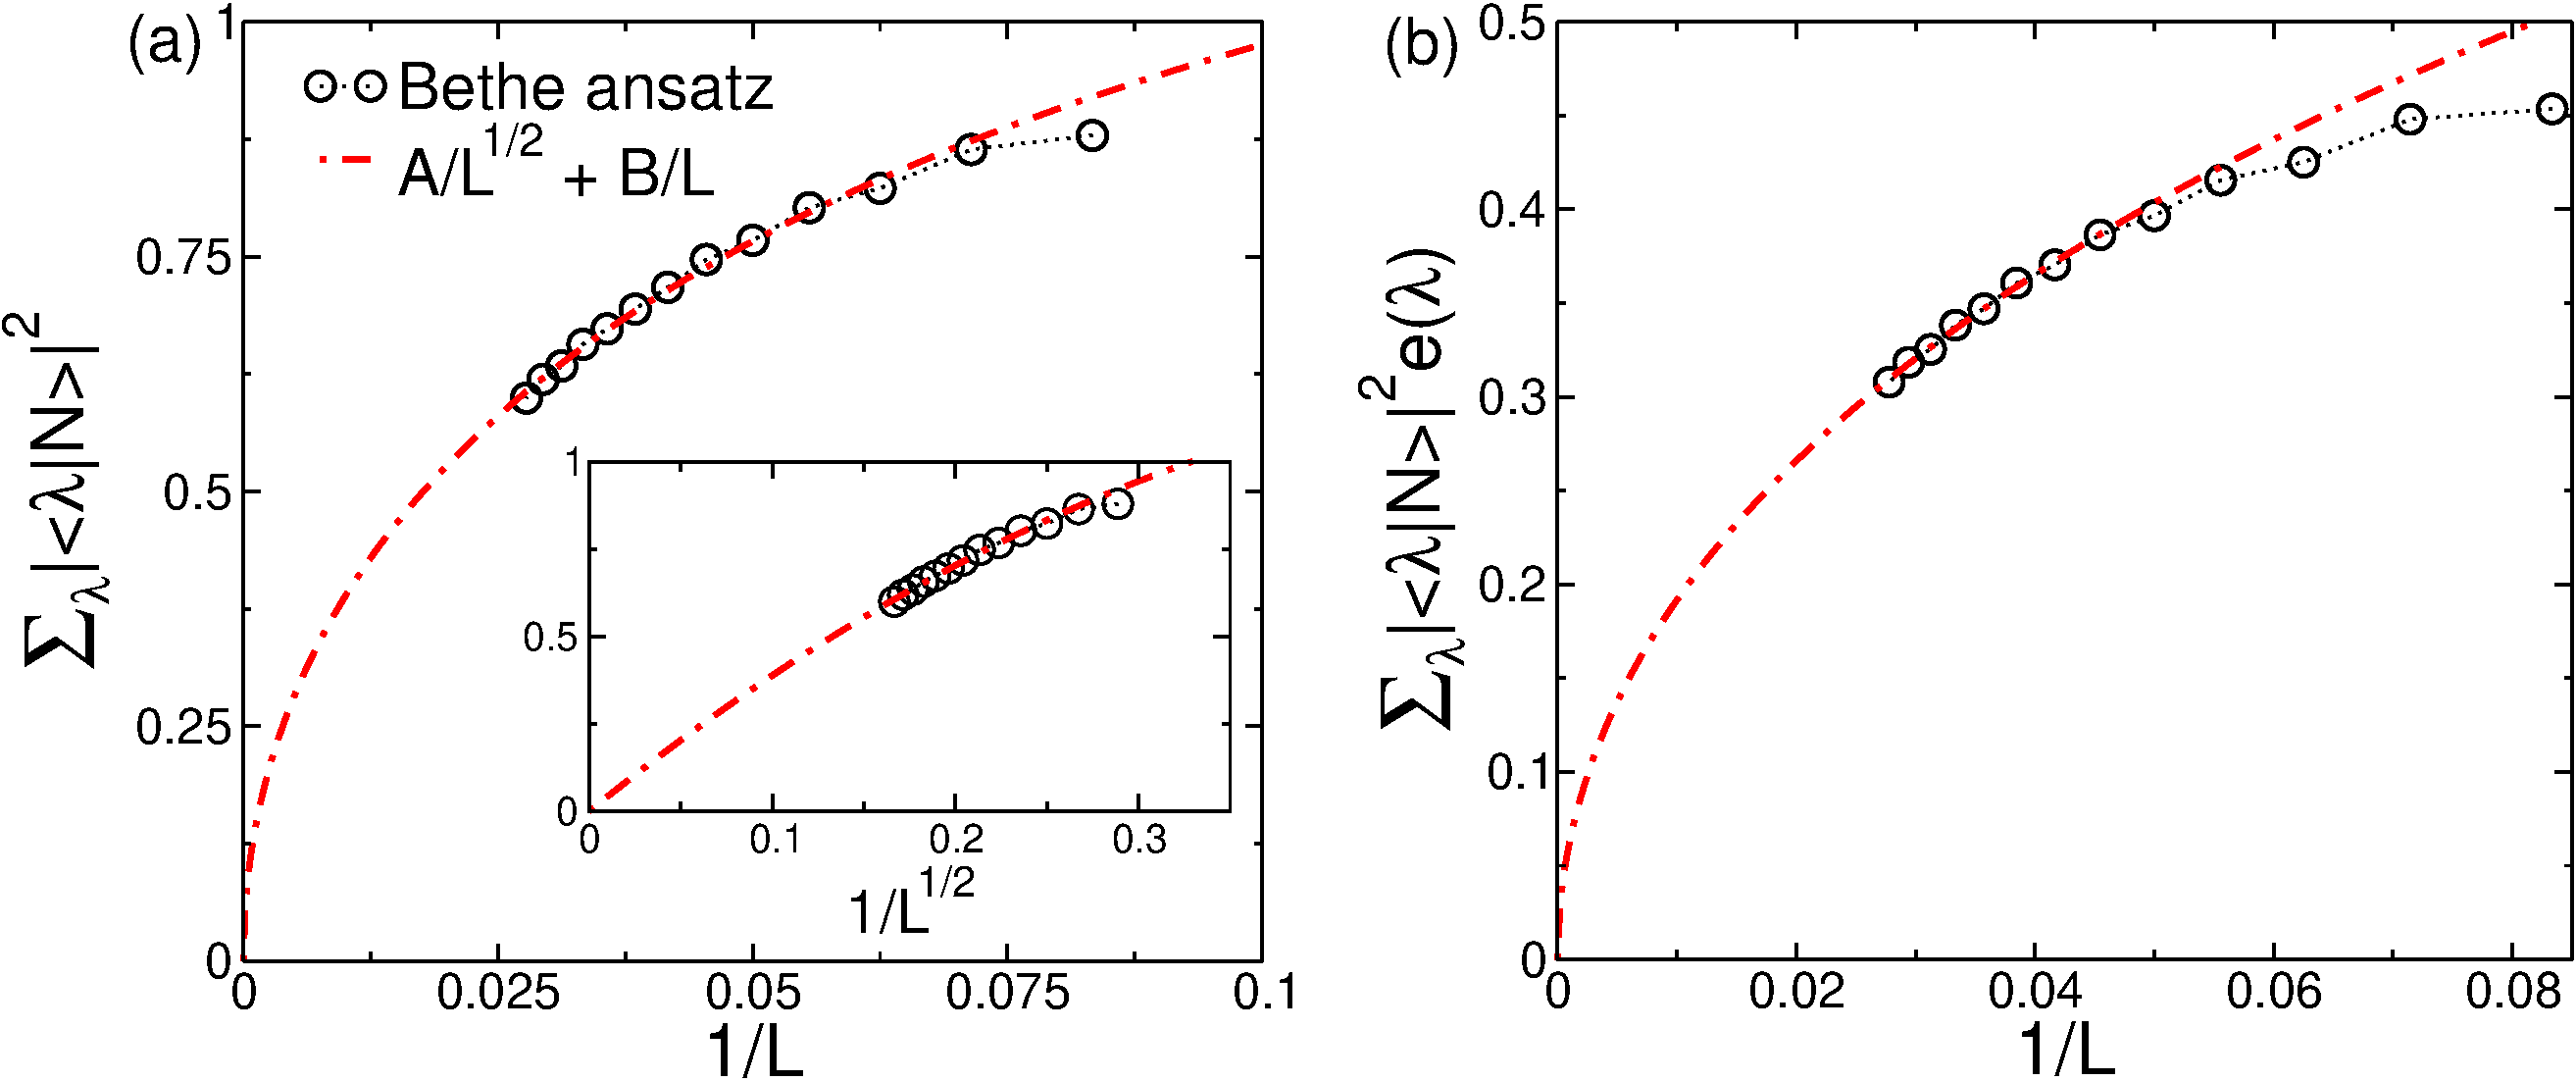
\includegraphics[width=.9\textwidth]{./draft_figs/Neel}
\end{center}
\caption{ Overlap sum rules for the Neel state: The role of the zero-momentum 
 strings. (a) The overlap sum rule $\sum_{\lambda}|\langle\lambda|N\rangle|^2=1$, 
 with $|N\rangle$ the Neel state and $|\lambda\rangle$ the eigenstates  of 
 the $XXX$ spin chain. The $x$-axis shows $1/L$, with $L$ the chain length. 
 The circles are Bethe ansatz results for chains up to $L=36$. The results 
 are obtained via a full scanning of the chain Hilbert space. Only the 
 eigenstates with no zero-momentum strings are considered. The dash-dotted 
 line is a fit to $A/L^{1/2}+B/L$, with $A,B$ fitting parameters. Inset: 
 The same data as in the main Figure plotted versus $1/L^{1/2}$. (b) 
 The same as in (a) for the sum rule $\sum_{\lambda}|\langle
 \lambda|N\rangle|^2e(\lambda)=1/2$, with $e(\lambda)$  the 
 eigenstates energy density. 
}
\label{fig1:neel-sr}
\end{figure}
%##################################################################

Here we investigate the effect of the Hilbert space truncation removed the 
zero-momentum strings on the N\'eel sum rules. 
We focus on the ``trivial'' sum rule, i.e., the normalization of the initial 
state 
%
\begin{equation}
\label{sr-trivial}
\langle N|N\rangle=\sum\limits_{\lambda}|\langle\lambda|N\rangle|^2=1, 
\end{equation}
%
and the local conserved charges sum rules 
%
\begin{equation}
\label{sr-charge}
Q_n^{(0)}=\langle N|Q_n|N\rangle=\sum\limits_{\lambda}|\langle\lambda|N\rangle|^2
q_{n}(\lambda)\quad\textrm{with}\quad n\in\mathbb{N}, 
\end{equation}
%
where $Q_n$ are the conserved charges of the $XXX$ chain (cf. 
subsection~\ref{sec:1.5}) and $q_n(\lambda)$ are the charges eigenvalues over 
the generic Bethe state $|\lambda\rangle$ (cf.~\eref{qngnk} and~\eref{gnk}). 

In~\eref{sr-charge} $Q_n^{(0)}$ is the charge expectation value over the initial 
state, i.e., the N\'eel state. These can be calculated as done in 
Ref.~\cite{fagotti-2013}. 

Note that due to the locality of $Q_n$, the translational invariance of the initial 
state, and the periodic boundary conditions, the charge density $Q_n^{(0)}/L$ does 
not depend on the chain size. For the N\'eel state, in the thermodynamic limit 
$Q_n^{(0)}$ is obtained using~\eref{q0-th} and the quench action root distributions 
$\pmb{\rho}^*$ (cf.~\eref{rho1-sp}-\eref{rho3-sp}). 

The truncation of the chain Hilbert space removing the zero-momentum strings has 
dramatic effects on the sum rules~\eref{sr-trivial} and~\eref{sr-charge}. 

This is illustrated in Figure~\ref{fig1:neel-sr} (a) focusing on the ``trivial'' 
sum rule~\eref{sr-trivial} and in Figure~\ref{fig1:neel-sr} (b) for~\eref{sr-charge} 
with $n=2$, i.e., the energy sum rule. 
For the N\'eel state, for any finite $L$ Eq.~\eref{sum} gives $Q^{(0)}_2/L=-1/2$. 

The circles in Figure~\ref{fig1:neel-sr} are the numerical results for the sum rules 
obtained via a full scanning of the Hilbert space of the Heisenberg chain, excluding 
the zero momentum strings. The data are plotted against the inverse chain length $1/L$, 
for $L\le 38$. The expected results including all the eigenstates are shown as 
horizonthal dotted lines in the Figure. 

Clearly, both the sum rules are violated, due to the exclusion of the to zero-momentum 
strings. Moreover, in both panesl the data suggest a vanishing behavior upon increasing 
the chain size. In particular, the dash-dotted lines in the Figures are fits to  
$A/L^{1/2}+B/L$, with $A,B$ fitting parameters, which perfectly describes the behavior 
of the data. 

The vanishing behavior as $\propto 1/L^{1/2}$ is reflecting the vanishing 
of the fraction of non-zero momentum string eigenstates in the thermodynamic limit.  
Precisely, from~\eref{zneel1} and~\eref{ztilde} one obtains 
%
\begin{equation}
\label{beh}
\frac{\widetilde Z_{Neel}}{Z_{Neel}}\propto\frac{4}{\sqrt{\pi L}}. 
\end{equation}
% 
in the thermodynamic limit. 

%##################################################################
\begin{figure}[t]
\begin{center}
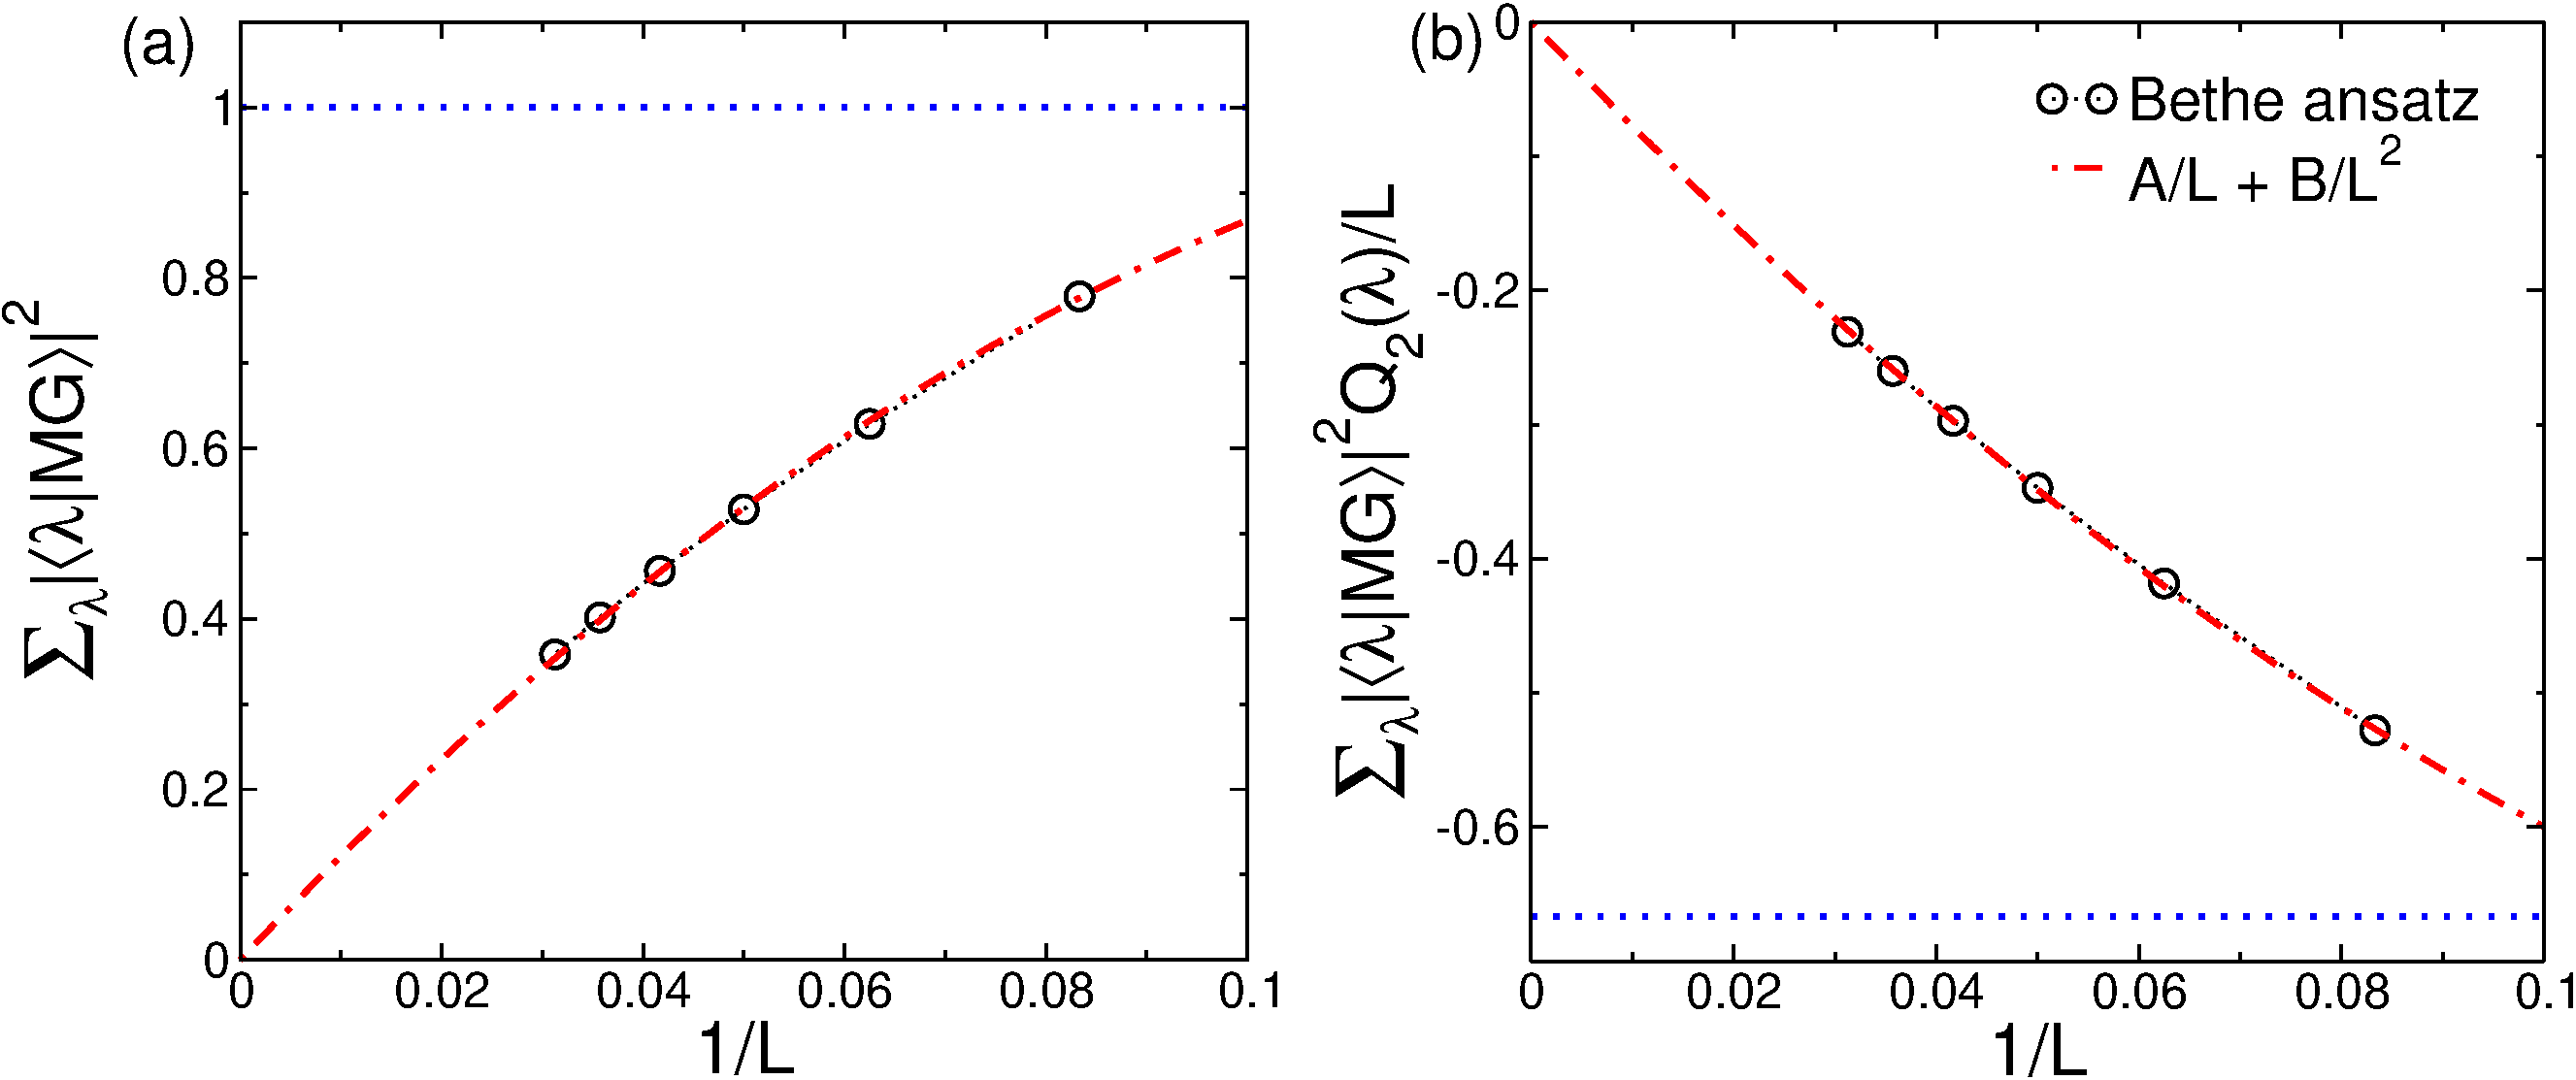
\includegraphics[width=.9\textwidth]{./draft_figs/Dimer}
\end{center}
\caption{ Overlap sum rules for the Majumdar-Ghosh (MG) state. (a) The 
 overlap sum rule $\sum_{\lambda}|\langle\lambda|MG\rangle|^2=1$, 
 with $|MG\rangle$ the Majumdar-Ghosh state and $|\lambda\rangle$ 
 the eigenstates  of the $XXX$ spin chain. The $x$-axis shows $1/L$, 
 with $L$ the chain length. The circles are Bethe ansatz results for 
 chains up to $L=36$. The results are obtained via a full scanning of 
 the chain Hilbert space. Only the eigenstates with no zero-momentum 
 strings are considered. The dash-dotted line is a fit to $A/L+B/L^2$, 
 with $A,B$ fitting parameters. (b) The same as in (a) for the sum 
 rule $\sum_{\lambda}|\langle\lambda|MG\rangle|^2e(\lambda)=
 2/3$, with $e(\lambda)\equiv E/L$  the eigenstates energy density. 
}
\label{fig2:dimer-sr}
\end{figure}
%##################################################################




The asymptotic, i.e., at large $L$, behavior as $1/\sqrt{L}$ is not generic, 
meaning that it depends on the initial state $|\Psi_0\rangle$. 
This is illustrated in Figure~\ref{fig2:dimer-sr}, focusing on the Majumdar-Ghosh 
(MG) state. Panels (a) and (b) plot are the same as in Figure~\ref{fig1:neel-sr}. 
The expected value for the energy density sum rule is $Q_2^{(0)}=-2/3$ (horizonthal dotted 
line in Figure~\ref{fig2:dimer-sr}). 
As for the N\'eel state only parity-invariant eigenstates containing no zero-momentum 
strings are consdidered. Note that their number $\widetilde Z_{MG}$ (cf.~\eref{mg-fi}) 
is now given as 
%
\begin{equation}
\widetilde Z_{MG}=B\Big(\frac{L}{2},\frac{L}{4}\Big)-B\Big(\frac{L}{2},
\frac{L}{4}-1\Big). 
\end{equation}
%
Similar to Figure~\ref{fig1:neel-sr}, due to the exclusion of the zero-momentum 
strings, the saturation rules exhibit vanishing behavior in the thermodynamic 
limit. However, in contrast with the N\'eel case, one has the behavior $\sim 1/L$, 
as confirmed by the fits (dash-dotted lines in Figure~\ref{fig2:dimer-sr}). 

Similar to the N\'eel case this reflects the same vanishing behavior of the 
eigenstates containing no zero-momentum strings $\widetilde Z_{MG}/Z_{MG}$ as 
%
\begin{equation}
\frac{\widetilde Z_{MG}}{Z_{MG}}=\frac{4}{4+L}. 
\end{equation}
%
where $Z_{MG}$ is the total number of parity-invariant eigenstates having non-zero 
overlap with the Majumdar-Ghosh state. 


%%%%%%%%%%%%%%%%%%%%%%%%%%%%%%%%%%%%%%%%%%%%%%%%%%%%%%%%%%%%%%%%%%%%%%%%%%%
\section{Monte Carlo implementation of the quench action approach}
\label{sec6:mcqa}

In this section follwing Ref.~\cite{alba-2015} we present the implementation of 
the quench action approach, focusing on the $XXX$ chain. The key idea is to sample 
the eigenstates of the finite-size $XXX$ 
chain with the quench action probability distribution given in~\eref{qa-d-ensemble}. 
Importantly, we restrict ourselves to the set of eigenstates of the $XXX$ chain 
with no zero-momentum strings. In subsection~\ref{sec:6.1} we introduce the Monte 
Carlo algorithm. Using the Monte Carlo algorithm in subsection~\ref{sec:6.2} we 
numerically demonstrates that the N\'eel sum rules~\eref{sr-charge} are recovered 
in the thermodynamic limit. The Hilbert space truncation is reflected in 
$\propto 1/L$ scaling corrections to the sum rules. Physically, this implies that 
despite the Hilbert space cut, the remaining eigenstates contain enough information 
to reproduce the correct physical behavior in the thermodynamic limit. 

In the Bethe ansatz framework this means that the eigenstates sampled by the Monte 
Carlo method approach the quench action representative state in the thermodynamic 
limit. This is explicitly demonstrated here by numerically calculating the 
quench action root distributions $\pmb{\rho}^*$, which are found in remarkable 
agreement with the analytical results. 



%%%%%%%%%%%%%%%%%%%%%%%%%%%%%%%%%%%%%%%%%%%%%%%%%%%%%%%%%%%%%%%%%%%%%%%%%%%
\subsection{Quench Action Monte Carlo algorithm}
\label{sec:6.1}


The Monte Carlo procedure starts with a randomly selected parity-invariant 
eigenstate (Bethe state) of the $XXX$ chain in the sector with zero magnetization, 
i.e., $M=L/2$ particles. 

Due to the fact that the N\'eel state is not invariant under $SU(2)$ rotations, 
to characterize the Bethe states one has to specify the number of infinite rapidities. 
Let us define the number of infinite rapidities $N_{\infty}$. Clearly, one has that 
the number of particles with finite rapidities $M'$ as $M'=L/2-N_\infty$. 
The state is identified by a parity-invariant Bethe quantum number 
configuration ${\mathcal C}$. Due to the parity-invariance and the fact that zero-momentum 
strings are excluded, the state is characterized by the number $m'$ of parity-invariant 
rapidity pairs $\{\pm\lambda_j\}_{j=1}^{m'}$. The string content 
associated with the finite rapidity pairs is denoted as $\widetilde{\mathcal S}=
\{\tilde s_1,\dots,\tilde s_{m'}\}$. The Monte Carlo procedure generates a new 
parity-invariant eigenstate of the $XXX$ chain, and it consists of four steps as 
follows: 
%
\begin{enumerate}
\item[\circled{1}] Choose a new number of finite rapidities $M_{new}'$ and a 
parity-invariant rapidity pairs $m_{new}'\equiv M_{new}'/2$ with 
probability ${\mathcal P}(M'_{new})$ as 
%
\begin{equation}
\label{PM}
{\mathcal P}(M'_{new})=\frac{\widetilde Z'_{Neel}(L,M'_{new})}
{\widetilde{Z}_{Neel}(L)}, 
\end{equation}
%
where $\widetilde Z_{Neel}(L)$ is the total number of parity-invariant eigenstates 
with no zero-momentum strings (cf.~\eref{ztilde}), and $\widetilde Z'_{Neel}$ is the 
number of parity invariant eigenstates with no zero-momentum strings in the 
sector with $M'_{new}$ particles with finite rapidities (cf.~\eref{neel-fi}). 
\item[\circled{2}] Choose a new a new string content $\widetilde{\mathcal S}'\equiv
\{\tilde s_1',\dots,\tilde s_{m'_{new}}\}$ with probability ${\mathcal P}'(M'_{new},
\widetilde{\mathcal S}')$
%
\begin{equation}
\label{PS}
{\mathcal P}'(M'_{new},\widetilde{\mathcal S}')=\frac{1}{\widetilde Z'_{Neel}
(L,M'_{new})}\prod_{n=1}^{m'_{new}}B\Big(\frac{L}{2}-\sum\limits_{l=1}^{
m'_{new}}t_{nl}\tilde s'_l,\tilde s'_n\Big), 
\end{equation}
%
where the matrix $t_{nl}$ is defined in~\eref{bt-qn-bound}.
\item[\circled{3}] Generate a new parity-invariant quantum number configuration 
${\mathcal C}'$ compatible with the $\widetilde {\mathcal  S}'$ obtained in step 
$\circled{2}$. Solve the corresponding BGT equations~\eref{bgt-eq}, finding the 
rapidities $\{\pm\lambda'_j\}_{j=1}^{m'_{new}}$ of the new parity-invariant 
eigenstate. 
\item[\circled{4}] Calculate the overlap $\langle\{\lambda'_j\}_{j=1}^{m'_{new}}
|N\rangle$ between the new eigenstate and the N\'eel state 
using~\eref{neel-ov}~\eref{red-G+}~\eref{red-G-} and~\eref{neel-k}. Accept the 
new eigenstate with the quench action Metropolis probability 
%
\begin{equation}
\label{metropolis}
{\mathcal P}''_{\lambda\to\lambda'}=\textrm{Min}\Big\{1,\exp\Big(-
2\Re({\mathcal E}'-{\mathcal E})\Big)\Big\}, 
\end{equation}
%
where ${\mathcal E}'\equiv-\log\langle\{\lambda'_j\}_{j=1}^{m'_{new}}
|N\rangle$, ${\mathcal E}\equiv-\log\langle\{\lambda_j\}_{j=1}^{m'_{new}}
|N\rangle$, and $\Re$ denoting the real part. 
\end{enumerate}
%
Note that while the steps $1$-$3$ generate the correct eigenstate energy density 
distribution, $4$ weigh the different eigenstates with the quench action probability 
distribution. 

For a generic observable ${\mathcal O}$, the long-time quench action value $\langle{
\mathcal O}\rangle$ is obtained as the arithmetic average of the expectation value 
over the eigenstates $|\lambda\rangle$ sampled by the Monte Carlo as 
%
\begin{equation}
\label{qamc-obs}
\langle{\mathcal O}\rangle=\frac{1}{N_{mcs}}\sum\limits_{\lambda}\langle\lambda|
{\mathcal O}|\lambda\rangle, 
\end{equation}
%
with $N_{mcs}$ being the total number of Monte Carlo steps. Note that, as usual in 
Monte Carlo, some initial steps have to be neglected to ensure thermalization. 
Note that~\eref{qamc-obs} applies to any observable ${\mathcal O}$ for which the 
the Bethe state expectation value $\langle\lambda|{\mathcal O}|\lambda\rangle$ 
(form factor) is known. 


%%%%%%%%%%%%%%%%%%%%%%%%%%%%%%%%%%%%%%%%%%%%%%%%%%%%%%%%%%%%%%%%%%%%%%%%%%%
\subsection{The N\'eel sum rules: Monte Carlo results}
\label{sec:6.2}

%##################################################################
\begin{figure}[t]
\begin{center}
\includegraphics[width=.9\textwidth]{./draft_figs/QAMC_Obs_Neel}
\end{center}
\caption{The overlap sum rules for the Neel state: Numerical results 
 obtained using the Hilbert space Monte Carlo sampling approach. (a) 
 The energy sum rule $\langle N|Q_2|N\rangle/L=-1/2$, with $Q_2/L$ 
 the Hamiltonian density. We plot $\sum_{\lambda}|\langle\lambda|
 N\rangle|^2Q_2(\lambda)/L=1/2$, with $|\lambda\rangle$ the 
 eigenstates of the $XXX$ chain, versus the inverse chain length $1/L$. 
 The symbols are Monte Carlo data obtained by sampling the eigenstates 
 of the $XXX$ chain. The dash-dotted line is the expected result. The 
 dashed line is a fit to the behavior $-1/2+A/L+B/L^2$, with $A,B$ 
 fitting parameters. (b) The energy fluctuations sum rule $\sigma^2(Q_2)/
 L\equiv(\langle N|Q_2^2|N\rangle-\langle N|Q_2|N\rangle^2)/L=1/4$. The 
 horizontal line is the expected result. (c)(d) Same as in (a)(b) for 
 the charge $Q_4$ and its fluctuations. 
}
\label{fig3:neel-qamc-sr}
\end{figure}
%##################################################################


The validity of the Monte Carlo approach for simulating the Quench-Action 
results is demonstrated in Figure~\ref{fig3:neel-qamc-sr}. The Figure focuses on 
the N\'eel sum rules for the conserved charges densities $Q_2/L$ and $Q_4/L$ 
(cf. subsection~\ref{sec:1.5} and~\eref{sr-charge}) and their fluctuations 
$\sigma(Q_n)$, which are defined as 
%
\begin{equation}
\fl\quad\sigma^2(Q_n)\equiv\langle N|Q^2_n|N\rangle-\langle N|Q_n|N\rangle^2=
\sum\limits_{\lambda}|\langle N|\lambda\rangle|^2q^2_n(\lambda)-\Big(\sum_\lambda|
\langle N|\lambda\rangle|^2q_n(\lambda)\Big)^2.
\end{equation}
%
Panel (a) and (b) in Figure~\ref{fig3:neel-qamc-sr} show the sum rules for 
the energy density $Q_2/L$, and its density of fluctutations $\sigma^2(Q_2)/L$. 
It is straightforward to derive the N\'eel expectation value of the energy 
density fluctuations as $\sigma(Q_2)/L=1/4$ (dash-dotted line in 
Figure~\ref{fig3:neel-qamc-sr} (b)). 

%Note that the N\'eel sum rule for the identity $\mathbb{I}$ is trivially satisfied, 
%and it corresponds to the normalization of the Monte Carlo probability. 
%Figure~\ref{fig5-neel-sr} (a) plots the N\'eel sum rule for the energy density $Q_2/L$. 
The circles in the Figure are Monte Carlo data obtained using the procedure outlined 
in~\ref{sec:6.1} for the Heisenberg spin chain with $L\le 56$ sites.  
The data correspond to Monte Carlo simulations with $N_{mcs}\sim 10^7$ Monte Carlo 
steps (mcs). For the largest chain size $L=56$ we used $N_{mcs}\sim ...$. The data 
are plotted versus inverse chain length $1/L$. 
%The expected result $\langle N|\hat Q_2|N\rangle/L=-1/2$ is shown as dash-dotted 
%line. 

Interestingly, the Monte Carlo data strongly suggest that in the thermodynamic limit 
the sum rule saturates are restored, while violations are present for finite chains. 
This numerically demonstrates that the truncation of the Hilbert space, i.e., 
removing the zero-momentum strings, gives rise to scaling corrections, while the 
thermodynamic limit behavior is correctly reproduced. 
Furthermore, the data in panel (a) suggest the behavior $\propto 1/L$ for the scaling 
corrections, as confirmed by the fit to $-1/2+A/L+b/L^2$ (dashed line in the Figure), 
with $A,B$ fitting parameters. 

The same behavior should be expected for the energy fluctuations $\sigma^2(Q_2)$, 
although this is difficult to extract numerically due to the large Monte Carlo 
error bar. 


Finally, panels (c) and (d) in Figure~\ref{fig3:neel-qamc-sr} are the same as 
(a)(b), but for the charge $Q_4$. While for $Q_4/L$ the Monte Carlo result 
for $L=48$ is already compatible with the expected result $Q_4/L=1/4$ in the 
thermodynamic limit, the scaling corrections of the fluctuations $\sigma^2(Q_4)$ 
are larger, and the Monte Carlo data show significant deviations from the 
thermodynamic limit up to $L=56$. 

This is explained that the support of $Q_4$, i.e., the number of sites where 
the operator acts non trivially is larger than for $Q_2$ (see~\cite{grabowski-1995} 
for the precise expression), and it is natural 
to assume that scaling corrections increase upon increasing the support of the 
operator considered. 

%%%%%%%%%%%%%%%%%%%%%%%%%%%%%%%%%%%%%%%%%%%%%%%%%%%%%%%%%%%%%%%%%%%%%%%%%%%
\subsection{The quench action root distributions}
\label{sec:6.3}

%##################################################################
\begin{figure}[t]
\begin{center}
\includegraphics[width=.95\textwidth]{./draft_figs/Neel_rho}
\end{center}
\caption{ The Quench-Action steady state root ddistributions $\rho_1(x)$ 
 and $\rho_2(x)$: Monte Carlos results. (a) The histograms of the $1$-string 
 rapidities sampled in the Monte Carlo. The $x$-axis shows the $1$-string BGT 
 root $\lambda$. The data are for a chain with $L=56$ sites and $N_{mcs}\sim 
 10^7$ Monte Carlo steps. The data are divided by a factor $10^6$ for plotting 
 convenience. The width of the histogram bin is $\Delta\lambda\sim 0.07$. (b) 
 The same as in (a) for the $2$-string roots sampled in the Monte Carlo. (b) 
 The extracted $1$-string root distribution $\rho_1(\lambda)$ plotted versus 
 $\lambda$ for two chains with $L=48$ and $L=56$ (diamond and circles, respectively). 
 The full line is the Quench-Action analytic result in the thermodynamic limit. (d) 
 The same as in (c) for the $2$-string root density $\rho_2(\lambda)$. In both 
 (c)(d) the oscillations are finite-size effects, whereas the error bars 
 show the statistical Monte Carlo error. 
}
\label{fig4:neel-rho}
\end{figure}
%##################################################################

The BGT root distributions corresponding to the quench action steady state 
(cf.~\eref{rho1-sp}-\eref{rho3-sp}) $\pmb{\rho}=\{\rho_n(\lambda)\}_{n=1}^{\infty}$ can be extracted 
from the Monte Carlo simulation.  This has been shown in Ref.~\cite{alba-2015} for 
the GGE representative state. 

The underlying idea is that for the local observables considered in this 
work the eigenstate expectation value $\langle\lambda|{\mathcal O}|\lambda\rangle$
entering in~\eref{qamc-obs} becomes
%
\begin{equation}
\langle\lambda|{\mathcal O}|\lambda\rangle=\sum\limits_{n,\gamma}{\mathcal O}
(\lambda_{n;\gamma}), 
\end{equation}
%
with the set of solutions of the BGT equations $\{\lambda_{n;\gamma}\}$ identifying 
the Bethe state $|\lambda\rangle$. 
By comparing~\eref{qamc-obs} and ... one obtains
%
\begin{equation}
\frac{1}{N_{mcs}}\sum\limits_{\{\lambda_{n;\gamma}\}}{\mathcal O}_n(\lambda_{n;\gamma})
\to\int_{-\infty}^{+\infty}d\lambda\rho_{n}(\lambda){\mathcal O}_n(\lambda). 
\end{equation}
%
This suggests that for any $n$ the histograms of the BGT roots corresponding to the 
$n$-strings sampled in the Monte Carlo should converge in the thermdynamic limit to 
the root distribution $\rho_n$. 

This is demonstrated numerically in Figure~\ref{fig4:neel-rho} for the first two root 
distributions $\rho^*_1(\lambda)$ (panel (a)(b)) and $\rho^*_2(\lambda)$ (panel 
(c)(d)). The data are obtained using the algorithm described in subsection~\ref{sec:6.1} 
for chains with up to $L\le 56$ sites. The data for $L=48$ correspond to a Monte Carlo 
history with $N_{mcs}\sim 10^7$ Monte Carlo steps (cf.~\eref{qamc-obs}), whereas we 
used $N_{mcs}\sim 10^8$ for $L=56$. 

Panel (a) and (c) show the  histograms of the $1$-string and $2$-string BGT roots sampled 
in the Monte Carlo, respectively for the chain with $L=56$ sites. The $y$-axis is 
divided by a factor $10^6$ for convenience. The width of the histogram bins $\Delta\lambda$ 
is $\Delta\lambda\approx0.02$ and $\Delta\lambda\approx0.001$ for $\rho_1(\lambda)$ 
and $\rho_2(\lambda)$, respectively. The histogram fluctuations are due both to the finite 
statistics (finite $N_{mcs}$) and to the finite size of the chain. 

The extracted quench action saddle point root distributions $\rho^*_1(\lambda)$ and 
$\rho^*(\lambda)$ are shown in panels (b) and (d). The data are the same as in panel 
(a)(c). The normalization of the histograms is chosen such as to match the analytical 
results from~\eref{rho1-sp} and~\eref{rho2-sp}, i.e., $\int d\lambda
\rho^*_1(\lambda)\approx0.31$ and $\int d\lambda\rho^*_2(\lambda)\approx
0.015$. The Monte Carlo error bars shown in the Figure are obtained with a standard 
jackknife analysis~\cite{quenouille-1949,wolff-2004}. 
The continuous lines are the expected analytic result in the thermodynamic limit given 
in~\eref{rho1-sp} and~\eref{rho2-sp}. 
Clearly, $\rho_1(\lambda)$ is in good agreement with the Monte Carlo data in the 
whole range $-2\le\lambda\le2$ considered. The statistical error bars are smaller 
than the symbol size. The oscillations are due to the finite size of the chain, and 
decrease with the chain size (see the data for $L=48$). 
On the other hand, larger (oscillating) finite size effects are observed for $\rho_2(\lambda)$. 
These deviations are larger on the tails of the root distribution. This is expected since 
large $\lambda$ correspond to large quasimomenta, which are more sensitive to the finite 
size of the chain. Moreover, the Monte Carlo error bars are clearly visible. This is 
due to the fact that since $\int d\lambda\rho^*_2(\lambda)/\sum_n\int d\lambda
\rho_n^*(\lambda)\approx 0.04$, the statistics available to estimate $\rho_2^*(\lambda)$ 
is effectively reduced as compared to $\rho_1^*(\lambda)$. 
Finally, we numerically checked that this effect is more dramatic for the longer strings 
root distribution, and larger statistics and larger chain would be needed already  
to extract $\rho_3(\lambda)$

%%%%%%%%%%%%%%%%%%%%%%%%%%%%%%%%%%%%%%%%%%%%%%%%%%%%%%%%%%%%%%%%%%%%%%%%%%%
\section{Conclusions}
\label{conclusions}

We presented a Monte Carlo implementation of the quench action method for integrable 
spin chains. We focused on the spin-$1/2$ isotropic Heisenberg spin chain ($XXX$ chain) 
and the quench from the zero-momentum N\'eel state. 
The approach extends the Monte Carlo approach developed in Ref.~\cite{alba-2015} to 
simulate the Generalized Gibbs Ensemble in integrable models. The key idea of the 
approach is the Monte Carlo sampling of the model Hilbert space with the quench 
action, equivalently the Diagonal Ensemble, probability distribution given 
in~\eref{qa-prob}. 

The approach is based on the knowledge of the 
overlaps between the pre-quench N\'eel state $|N\rangle$ and the eigenstates 
of the model that have been obtained recently~\cite{pozsgay-2014,brockmann-2014,
brockmann-2014a,brockmann-2014b,brockmann-2014c,piroli-2014}. 

Besides the overlaps the method is based on the knowledge of the Hilbert space 
structure provided by the Bethe ansatz formalism and on the Bethe-Gaudin-Takahashi 
(BGT) equations. The approach is devised for finite-size systems. Thermodynamic 
quantities can be extracted using finite-size scaling. 

We first focused on the importance of the so-called zero-momentum strings. 
These corresponds to components of the Bethe wavefunctions corresponding to 
bound states of many down spins (strings in the Bethe ansatz language) with 
zero center of mass momentum. These are usually neglected in the quench action 
approach~\cite{brockmann-2014}. The reason is that zero momentum strings 
leads to singularities in the overlap formulas, which make extracting the 
thermodynamic limit tricky. Moreover, it is argued that zero-momentum 
strings give rise only to scaling corrections to the quench action results, 
which are unimportant in the thermodynamic limit. 

Importantly, one should observe that for a finite chain the vast majority of 
eigenstates contain zero-momentum strings. More precisely, for the quench from 
the N\'eel state the fraction of eigenstates with no zero-momentum strings 
vanish as $\propto L^{-1/2}$. 

Moreover, the only eigenstates having non zero N\'eel overlaps (and non zero 
overlap with the Majumdhar-Ghosh state) are the so-called parity invariant 
eigenstates. The total number of parity-invariant eigenstates of the Heisenberg 
spin chain is given in terms of the chain length by a simple combinatorial 
formula that we provide. We provide similar combinatorial formulas for the 
total number of parity-invariant eigenstates at fixed number of down spins 
and fixed string content, i.e., the number of many-spin bound states present in 
each eigenstates. 

In order to understand the importance of the zero-momentum strings we calculated 
the overlap distribution function including all the eigenstates of the chain for 
chains up to $L=38$ sites. We excluded the zero-momentum strings. 

We focused on some exact sum rules for the local integrals of motion of the 
$XXX$ chain. Strikingly, the exclusion of the zero momentum strings gives rise 
to violations of the sum rules. Precisely, we numerically observe that the 
sum rules exhibit the vanishing behavior $\propto L^{-\frac{1}{2}}$, which 
reflects the vanishing of the fraction of eigenstates with no zero-momentum 
strings. 

The behavior $\propto L^{-\frac{1}{2}}$ is not generic, but it depends on the 
pre-quench initial state. We demonstrated that by considering the quench from 
the Majumdar-Ghosh state. We observed that the sum rule vanish as $1/L$, again 
reflecting the vanishing as $1/L$ of the fraction of eigenstates with no 
zero-momentum strings. 

We observed that the vast majority of the eigenstates have neglegible overlap 
with the N\'eel state. This implies that the eigenstates relevant for the 
quench action are a small fraction of the total number of eingestates having 
in principle non-zero N\'eel overlap. 

Next we presented a Monte Carlo implementation of the quench action method. 
This is obtained by resampling with the quench action probability measure 
the Hilbert space of the $XXX$ chain, restricted to the sector of the  Hilbert 
space with no zero-momentum strings. 

This is obtained using a standard Metropolis algorithm. Importantly, we 
numerically demonstrated that the only consequence of the Hilbert space 
restriction to strings with finite momentum are scaling corrections $1/L$ 
to physical observables. 

Specifically, we focused on the sum rules for the local conserved quantities 
of the $XXX$ chain. We numerically observed that, although for finite chains 
violations of the sum rules are present, these violations decay upon increasing 
the chain size, and the sum rules are restored in the thermodynamic limit. 

Finally, we extracted from the Monte Carlo the BGT root distributions characterizing 
the quench action saddle point. These are obtained from the BGT roots identifying 
the $XXX$ chain eigenstates sampled in the Monte Carlo. We observed that, although 
the finite size gives rise to oscillating scaling corrections, already for 
relatively small chains with $L=56$ sites, the first BGT root distribution 
$\rho^*_1(\lambda)$ is in impressive agreement with the analytic result in 
the thermodynamic limit. 



\appendix

%%%%%%%%%%%%%%%%%%%%%%%%%%%%%%%%%%%%%%%%%%%%%%%%%%%%%%%%%%%%%%%%%%%%%%%%%%%
\section{Eigenstates with nonzero N\'eel overlap: eigenstates counting and 
string content}
\label{app-1}

Here we prove that the total number of eigenstates with N\'eel nozero overlap 
$Z_{Neel}(L)$for a chain of length $L$ is given as 
%
\begin{equation}
\label{N-count}
Z_{Neel}=2^{\frac{L}{2}-1}+\frac{1}{2}B\Big(\frac{L}{2},\frac{L}{4}\Big)+1. 
\end{equation}
%
For simplicity here we restrict ourselves to the situation with $L$ divisible by 
four. The strategy to prove~\eref{N-count} is to count all the possible parity-invariant 
BGT quantum numbers configurations. Let us consider the sector with fixed number of 
particles $M$, and a generic string content ${\mathcal S}=\{s_1,s_2,\dots,s_{M}\}$. 
Here $s_n$ is the number of $n$-strings, and one has the constraint $\sum_k ks_k=M$. 

It is straightforward to check that total number of parity-invariant quantum number 
pairs ${\mathcal N}_n(L,{\mathcal S})$ in the $n$-string sector is given as 
%
\begin{equation}
\label{NnLS}
{\mathcal N}_n(L,{\mathcal S})=\Big\lfloor\frac{L}{2}-\frac{1}{2}
\sum_{m=1}^{M}t_{nm}s_m\Big\rfloor.
\end{equation}
%
where $t_{nm}\equiv 2\textrm{Min}(n,m)-\delta_{n,m}$. The number of parity-invariant 
quantum number configurations (i.e., eigenstates) ${\mathcal N}(L,{\mathcal S})$ 
compatible with string content ${\mathcal S}$ is obtained by choosing in all the 
possible ways the parity-invariant quantum number pairs independently in each 
$n$-string sector, which implies that    
%
\begin{equation}
\label{NLS}
{\mathcal N}(L,{\mathcal S})=\prod_{m=1}^{M} B\left({\mathcal N}_m,\left\lfloor
\frac{s_m}{2}\right\rfloor\right).
\end{equation}
%
Here the product is because each string sector is treated independently, while the 
factor $1/2$ in $s_m/2$ is because since all quantum numbers are organized in pairs, 
only half of the quantum numbers have to be specified. Note that in each $n$-string 
sector only one zero momentum (i.e., zero quantum number) string is allowed, due to 
the Pauli principle. Moreover, $s_m$ is odd (even) only if the zero momentum string 
is (not) present. The floor function $\lfloor\cdot\rfloor$ in~\eref{NLS} reflects 
that the quantum number of zero-momentum strings is fixed. 

We now consider the string configurations with particle number $0\le\ell\le M$ and 
fixed number of strings $1\le q\le M/2$. Note that the maximul allowed string length 
is $M/2$ beacause of parity invariance. Note also that in determining $q$ strings of 
different length are treated equally. Clearly, one has that $\sum_m s_m=q$. 
For a given fixed pair $\ell,q$ the total number of quantum number configurations 
is given as 
%
\begin{equation}
\label{NLlq}
{\mathcal N}'(L,\ell,q)=\sum\limits_{\{\{s_m\}\,:\, \sum m s_m=\ell, \sum s_m=q\}}
{\mathcal N}(L,{\mathcal S}),
\end{equation}
%
where the sum is over the content $\{s_m\}_{m=1}^M$ compatible with the constraints 
$\sum_m s_m=q$ and $\sum_m m s_m=\ell$. The strategy is to write a recursive relation 
for ${\mathcal N}'(L,\ell,q)$. To this purpose it is useful to consider the shifted 
string content ${\mathcal S}'$ defined as  
%
\begin{equation}
{\mathcal S}'\equiv \{s_{m+1}\}\quad\textrm{with}\, s_m\in{\mathcal S},\,\forall m.
\end{equation}
%
Using the definition of $t_{ij}$, it is straightforward to derive that  
%
\begin{equation}
t_{ij}=t_{i-1,j-1}+2,
\end{equation}
%
which implies that ${\mathcal N}_n(L,{\mathcal S})$ (see~\eref{NnLS}) satisfies the 
recursive equation 
%
\begin{equation}
{\mathcal N}_n(L,{\mathcal S})={\mathcal N}_{n-1}(L-2q,{\mathcal S}'). 
\end{equation}
%
After substituting in~\eref{NLS} one obtains 
%
\begin{equation}
\label{NLSr}
{\mathcal N}(L,{\mathcal S})=B\Big({\mathcal N}_1(L,{\mathcal S}),\Big\lfloor \frac{s_1}{2}
\Big\rfloor\Big){\mathcal N}(L-2q,{\mathcal S}'). 
\end{equation}
%
Finally, after substituting~\eref{NLSr} in~\eref{NLlq}, one obtains a recursive relation 
for ${\mathcal N}'(L,\ell,q)$ as 
%
\begin{equation}
\label{NpLlq}
{\mathcal N}'(L,\ell,q)=\sum_{s=0}^{q-1}B\Big(\frac{L}{2}-q+\Big\lfloor\frac{s}{2}\Big\rfloor,
\left\lfloor\frac{s}{2}\right\rfloor\Big){\mathcal N}'\left(L-2q,\ell-q,
q-s\right), 
\end{equation}
%
with the constraint that when $\ell=q$ one has 
%
\begin{equation}
{\mathcal N}'(L,q,q)=B\Big(\Big\lfloor\frac{L-q}{2}\Big\rfloor,\Big\lfloor\frac{q}{2} 
\Big\rfloor\Big).
\end{equation}
%
This is obtained by observing that if $\ell=q$ only $1$-strings are allowed and~\eref{NnLS} 
gives ${\mathcal N}_n(L,{\mathcal S})=\lfloor (L-q)/2\rfloor$. 

It is straightforward to check that for even $q$ the ansatz 
%
\begin{equation}
{\mathcal N}'(L,\ell,q)=\frac{q}{\ell}B\Big(\frac{L-\ell}{2},\frac{q}{2}\Big)
B\Big(\frac{\ell}{2},\frac{q}{2}\Big),
\end{equation}
% 
satisfies~\eref{NpLlq}. For odd $q$ the solution of~\eref{NpLlq} is 
%
\begin{equation}
{\mathcal N}'(L,\ell,q)=\frac{\ell-q+1}{\ell}B\Big(\frac{L-\ell}{2},\frac{q-1}{2}
\Big)B\Big(\frac{\ell}{2},\frac{q-1}{2}\Big).
\end{equation}
%
The number of eigenstates in the sector with $\ell$ particles with nonzero 
N\'eel overlap $Z'_{Neel}(L,\ell)$ are obtained by summing over all possible values 
of $q$ as 
%
\begin{equation}
\label{sum1}
Z'_{Neel}(L,\ell)=\sum\limits_{q=1}^\ell {\mathcal N}'(L,\ell,q).
\end{equation}
%
It is convenient to split the summation in~\eref{sum1} considering odd values of $q$ 
and even $q$ separately. For odd $q$ one obtains 
%
\begin{equation}
\sum\limits_{k=0}^{\ell/2-1} {\mathcal N}'(L,\ell,2k+1)=B\Big(\frac{L}{2}-1,
\frac{\ell}{2}-1\Big),
\end{equation}
%
while for even $q$ one has 
%
\begin{equation}
\sum\limits_{k=0}^{\ell/2} {\mathcal N}'(L,\ell,2k)=B\Big(\frac{L}{2}-1,
\frac{\ell}{2}\Big). 
\end{equation}
%
Putting everything together one obtains 
%
\begin{equation}
\label{N-count-p}
Z'_{Neel}(L,\ell)=B\Big(\frac{L}{2}-1,
\frac{\ell}{2}-1\Big)+B\Big(\frac{L}{2}-1,
\frac{\ell}{2}\Big). 
\end{equation}
%
The total number of eigenstates with nonzero N\'eel overlap $Z_{Neel}(L)$ 
(cf.~\eref{N-count}) is obtained from~\eref{N-count-p} by summing over 
the allowed values of $\ell=2k$ with $k=0,1,\dots,\ell/2$. 

Note that the total number $Z_{MG}$ of parity-invariant eigenstates having non 
zero overlap with the Majumdar-Ghosh state is obtained from Eq~\eref{N-count-p} 
replacing $\ell=L/2$, to obtain 
%
\begin{equation}
\label{p-inv-mg}
Z_{MG}=B\Big(\frac{L}{2}-1,\frac{L}{4}-1\Big)+B\Big(\frac{L}{2}-1,\frac{L}{4}
\Big). 
\end{equation}
%
Physically, this is due to the fact that the 
Majumdar-Ghosh state is invariant under $SU(2)$ rotations, which implies 
that only eigenstates with zero total spin $S=0$ can have non zero overlap. 


%%%%%%%%%%%%%%%%%%%%%%%%%%%%%%%%%%%%%%%%%%%%%%%%%%%%%%%%%%%%%%%%%%%%%%%%%%%
\section{Excluding the zero-momentum strings}
\label{app-2}

Here we demonstrate that the total number of eigenstates with nonzero N\'eel overlap, 
which do not contain zero-momentum strings, $\widetilde Z_{Neel}(L)$ is given as 
%
\begin{equation}
\widetilde Z_{Neel}(L)=B\Big(\frac{L}{2},\frac{L}{4}\Big). 
\end{equation}
%
Given a generic $M$-particle eigenstate of the $XXX$ chain, due to parity invariance, 
if one excludes the zero-momentum strings only $n$-strings with length $n\le M/2$ 
are allowed. Similarly, the string content is of the form $\widetilde{\mathcal S}
\equiv\{\tilde s_1,\dots,\tilde s_{M/2}\}$, i.e., $\tilde s_m=0$ $\forall m>M/2$.
Note that due to parity invariance and to the exclusion of the zero-momentum strings 
one has that $\tilde s_m$ is always an even integer. Clearly one has $\sum_{m=1}^{M/2}
m \tilde s_m=M$. 

The total number of parity-invariant quantum numbers $\widetilde{\mathcal N}_n$ in the 
$n$-string sector is given as  
%
\begin{equation}
\widetilde{\mathcal N}_n(L,\widetilde{\mathcal S})=\frac{L}{2}-\frac{1}{2}
\sum_{m=1}^{M/2}t_{nm}\tilde s_m.
\end{equation}
%
The proof now proceeds as in~\ref{app-1}. One can define the total number of eigenstates 
with nonzero N\'eel overla in the sector with $\ell$ particles and $q$ different strings as 
$\widetilde{\mathcal N}'(L,\ell,q)$. Note that due to parity invariance and the exclusion of 
zero-momentum strings, $q$ must be even. It is straigtforward to show that $\widetilde
{\mathcal N}'(L,\ell,q)$ obeys the recursive relation
%
\begin{equation}
\label{NpLlq-1}
\widetilde{\mathcal N}'(L,\ell,q)=\sum_{s=0}^{q/2-1}B\Big(\frac{L}{2}-q+s,s\Big)\widetilde
{\mathcal N}'\Big(L-2q,\frac{\ell-q}{2},\frac{q}{2}-s\Big),
\end{equation}
% 
with the constraint
%
\begin{equation}
\widetilde{\mathcal N}'(L,1,1)=\frac{L}{2}-1. 
\end{equation}
%
It is straightforward to check that the solution of~\eref{NpLlq-1} is given as 
%
\begin{equation}
\widetilde{\mathcal N}'(L,\ell,q)=\frac{L-2\ell+2}{L-\ell+2}B\Big(\frac{L-\ell}{2}+1,q\Big)
B\Big(\frac{\ell}{2}-1,\frac{q}{2}-1\Big).
\end{equation}
%
After summing over the allowed values of $q=2k$ with $k=1,2,\dots,\ell/2$ one obtains 
the total number of eigenstaets with nonzero N\'eel overlap at fixed number of 
particles $\ell$ $\widetilde Z_{Neel}'(L,\ell)$ as 
%
\begin{equation}
\label{neel-fi}
\widetilde Z_{Neel}'(L,\ell)=B\Big(\frac{L}{2},\frac{\ell}{2}\Big)-
B\Big(\frac{L}{2},\frac{\ell}{2}-1\Big).
\end{equation}
%
Summing over $\ell$ one obtains~\eref{neel-ov-count}.
Similar to~\eref{p-inv-mg} the total number of eigenstates $\widetilde Z_{MG}$ 
with no zero-momentum strings having non-zero overlap with the Majumdar-Ghosh 
state is obtained from~\eref{neel-fi} replacing $\ell\to L/2$, to obtain 
%
\begin{equation}
\label{mg-fi}
\widetilde Z_{MG}=B\Big(\frac{L}{2},\frac{L}{4}\Big)-B\Big(\frac{L}{2},\frac{L}{4}-1
\Big). 
\end{equation}
%
Interestingly, using~\eref{p-inv-mg} and~\eref{mg-fi}, one obtains that the ratio 
$\widetilde Z_{MG}/Z_{MG}$ is given as 
%
\begin{equation}
\frac{\widetilde Z_{MG}}{Z_{MG}}=\frac{4}{4+L}. 
\end{equation}
%


%%%%%%%%%%%%%%%%%%%%%%%%%%%%%%%%%%%%%%%%%%%%%%%%%%%%%%%%%%%%%%%%%%%%%%%%%%%
\section{Exact N\'eel and Majumdar-Ghosh overlaps for a small Heisenberg chain} 
\label{app-L12}

In this section we provide exact diagonalization results for the overlap of both the 
N\'eel state and the Majumdar-Ghosh (MG) state with all the eigenstates of the Heisenberg 
spin chain with $L=12$ sites. We also provide the corresponding results obtained 
using the string hypothesis and the overlap formulas~\eref{neel-ov} and~\eref{mg-ov}, 
restricting ourselves to eigenstates with no zero-momentum strings. 

%%%%%%%%%%%%%%%%%%%%%%%%%%%%%%%%%%%%%%%%%%%%%%%%%%%%%%%%%%%%%%%%%%%%%%%%%%%
\subsection{N\'eel overlap}
\label{app-neel}

The overlaps between all the eigenstates of the Heisenberg spin chain and the N\'eel 
state are reported in Table~\ref{table:neel}. The first column in the Table shows 
the string content ${\mathcal S}\equiv\{s_1,\dots,s_M\}$, with $M$ being the number 
of finite rapidities. The number of infinite rapidities $N_{\infty}=L/2-M$ is also 
reported. Note that eigenstates containing infinite rapidities correspond to 
different $S_z$ eigenvalue. The second column shows 
$2I_n^+$, with $I_n$ the Bethe-Gaudin-Takahashi quantum number identifying the 
BGT rapidity of the $n$-string. Due to the parity invariance only the positive 
quantum numbers are reported. The total number of independent strings, i.e., 
$q\equiv\sum_js_j$, is reported in the third column. The fourth column is the 
eigenstate's energy eigenvalue $E$. The last two columns show the squared N\'eel 
overlaps and the corresponding result obtained using the Bethe-Gaudin-Takahashi 
equations, respectively. In the last column only the case with no zero-momentum 
strings is considered. The deviations from the exact diagonalization results (digits 
with different colors) have to be attributed to the string hypothesis. Notice that  
the overlap between the N\'eel state and the $S_z=0$ eigenstate in the sector with 
maximal total spin $S=L/2$ (first column in Table~\ref{table:neel}), is given 
analytically as $2/B(L,L/2)$, with $B(x,y)$ the Newton binomial. 

Figure~\ref{fig1-BGT-check} plots the squared overlaps $|\langle\lambda|
N\rangle|^2$ between the N\'eel state and the eigenstates of the chain. 
The overlaps are plotted against the eigenstate energy density $E/L
\in[-\log(2),0]$. The circles are exact diagonalization results for all 
the chain eigenstates ($382$ eigenstates), whereas the crosses denote the 
overlaps calculated using formula~\eref{neel-ov}, and the 
Bethe-Gaudin-Takahashi equations. Note that only the eigenstates with 
no zero-momentum strings are shown ($252$ eigenstates) in the Figure. 
Panel (a) in the Figure is an overview of all the results. Panels (b)-(d) 
correspond to zooming to the smaller overlap values $|\langle N|\lambda
\rangle|\lesssim 0.02$, $|\langle N|\lambda\rangle|\lesssim 0.002$, and 
$|\langle N|\lambda\rangle|\lesssim 10^{-5}$. 

Clearly, the overlaps decay rapidly upon increasing the energy density. 
This is expected since the $XXX$ Hamiltonian expectation value over 
the N\'eel state is $\langle N|{H}|N\rangle=-1/2$. Importantly, the 
agreement between the exact diagonalization results and the results 
obtained using the BGT equations~\eref{ba_eq} is excellent, confirming 
the validity of the string hypothesis. 

%%%%%%%%%%%%%%%%%%%%%%%%%%%%%%%%%%%%%%%%%%
\begin{table}[h]
\scriptsize
\centering
Bethe states with nonzero N\'eel overlap ($L=12$)\\[1ex]
\begin{tabular}{rrrrrr}
\toprule
String content & $2I^+_n$ & $q$ & E & $|\langle\lambda|N\rangle|^2$ (exact) & $|\langle
\lambda|N\rangle|^2$ (BGT) \\[0.3em]
\toprule
6 inf & - & - & $0$ & $0.002164502165$ & $0.002164502165$\\
\midrule
\{2,0\}\, 4 inf &$1_1$ & $2$ & $-3.918985947229$ & $0.096183409244$ & $0.096183409244$\\
 &$3_1 $ & & $-3.309721467891$ & $0.011288497947$ &             $0.011288497947$\\
 &$5_1 $ & & $-2.284629676547$ & $0.004542580506$ &             $0.004542580506$\\
 &$7_1 $ & & $-1.169169973996$ & $0.002752622983$ &             $0.002752622983$\\
 &$9_1 $ & & $-0.317492934338$ & $0.002116006203$ &             $0.002116006203$\\
\midrule
\{4,0,0,0\}\, 2 inf &$1_1 3_1 $ & $4$ & $-7.070529325964$ & $0.310133033838$ &$0.310133033838$\\
  &$1_1 5_1 $ & & $-5.847128730477$ & $0.129277023687$ &           $0.129277023687$\\
  &$ 1_1 7_1$ & & $-4.570746557876$ & $0.085992436024$ &           $0.085992436024$\\
  &$ 3_1 5_1$ & & $-5.153853093221$ & $0.015256395523$ &           $0.015256395523$\\
  &$3_1 7_1 $ & & $-3.916336243695$ & $0.010091113504$ &           $0.010091113504$\\
  &$5_1 7_1 $ & & $-2.817696043731$ & $0.004059780228$ &           $0.004059780228$\\
\midrule
\{0,2,0,0\}\, 2 inf &$1_2 $ & $2$ & $-1.905667167442$ & $0.001207238321$ & $0.0012072{\color{red}45406}$\\
  &$3_2 $ & & $-1.368837200825$ & $0.002340453815$ &            $0.0023{\color{red}25724713}$\\
  &$5_2 $ & & $-0.681173793635$ & $0.001921010489$ &            $0.0019{\color{red}39001396}$\\
\midrule
\{1,0,1,0\}\, 2 inf &$0_1 0_3$ & $2$ & $-2.668031843135$ & $0.034959609810$ & -\\
\midrule
\{6,0,0,0,0,0\}\, 0 inf &$1_1 3_1 5_1$ & $6$ & $-8.387390917445$ & $0.153412152966$ & $0.153412152966$\\
\midrule
\{2,2,0,0,0,0\}\, 0 inf &$1_1 1_2$ & $4$ & $-5.401838225870$ & $0.040162686361$ & $0.04{\color{red}1042488913}$\\  
&$3_1 1_2 $ & & $-4.613929948329$ & $0.004636541934$ & $0.004{\color{red}730512604}$\\
  &$5_1 1_2 $ &  & $-3.147465758841$ & $0.001335522556$ & $0.00133{\color{red}7334035}$\\
\midrule
\{3,0,1,0,0,0\}\, 0 inf &$0_1 2_1 0_3$ & $4$ & $-6.340207488736$ & $0.052743525774$ & -\\
  &$0_1 4_1 0_3$ & & $-5.203653009936$ & $0.015022005621$ & - \\
  &$0_1 6_1 0_3$ & & $-3.788693957250$ & $0.011144489334$ & - \\
\midrule
\{1,0,0,0,1,0\}\, 0 inf &$0_1 0_5$ & $2$ & $-2.444293750583$ & $0.005887902992$ & - \\
\midrule
\{0,0,2,0,0,0\}\, 0 inf &$1_3$ & $2$ & $-1.111855930538$ & $0.001342476001$ & $0.0013{\color{red}84980817}$ \\
\midrule
\{0,1,0,1,0,0\}\, 0 inf &$0_2 0_4$ & $2$ &  $-1.560671012472$ & $0.000026982174$ & - \\
\bottomrule
\end{tabular}
\caption{All Bethe states for $L=12$ having nonzero overlap with the zero-momentum N\'eel state. 
 The first column shows the string content of the Bethe states, including the number of infinite 
 rapidities. The second and third column show $2I_n^+$, with $I_n^+$ the BGT quantum numbers 
 identifying the different states, and the number $q$ of independent strings. In the second 
 column only the positive BGT numbers are shown. The fourth column is the Bethe state eigenenergy. 
 Finally, the last two columns show the exact overlap with the N\'eel state and the approximate 
 result obatained using the BGT equations. In the last column Bethe states containing zero-momentum 
 strings are excluded. Deviations from the exact result (digits with different colors) are 
 attributed to the string hypothesis. 
}
\label{table:neel}
\end{table}
%%%%%%%%%%%%%%%%%%%%%%%%%%%%%%%%%%%%%%%%%%


%##################################################################
\begin{figure}[t]
\begin{center}
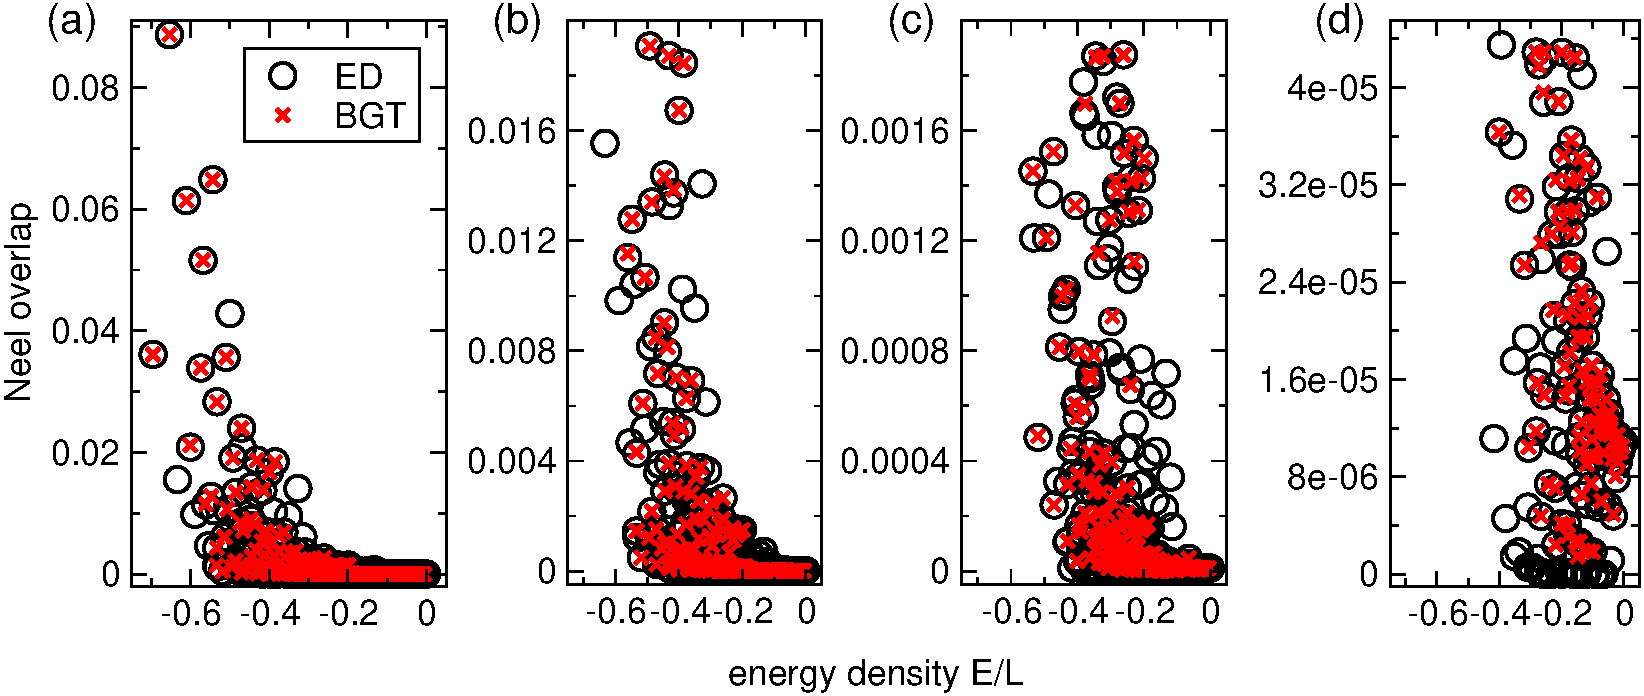
\includegraphics[width=.9\textwidth]{./draft_figs/L20_BT_check}
\end{center}
\caption{ The squared overlap $|\langle N|\lambda\rangle|^2$ between the the 
 Neel state $|N\rangle$ and the eigenstates $|\lambda\rangle$ of the $XXX$ 
 chain with $L=20$ sites. Only non-zero overlaps are shown. In all the panels the 
 $x$-axis shows the eigenstate energy density $E/L$. The circles are the exact 
 diagonalization results for all the non-zero overlaps. The crosses are the Bethe 
 ansatz results obtained using the Bethe-Gaudin-Takahashi equations. The missing 
 crosses correspond to eigenstates containing zero-momentum strings. (a) Overview 
 of all the non-zero overlaps. (b)(c)(d) The same overlaps as in (a) zooming in 
 the regions $[0,0.2]$, $[0,0.020]$, and $[0,4\cdot 10^{-5}]$. The discrepancies 
 between the ED and the Bethe ansatz results are attributed to the string 
 deviations. 
}
\label{fig1-BGT-check}
\end{figure}
%##################################################################

%%%%%%%%%%%%%%%%%%%%%%%%%%%%%%%%%%%%%%%%%%%%%%%%%%%%%%%%%%%%%%%%%%%%%%%%%%%
\subsection{Majumdar-Ghosh overlap}
\label{app-mg}
The overlap between the Heisenberg chain eigenstates with the Majumdar-Ghosh state are shown in 
Table~\ref{table:mg}. The conventions on the representation of the eigenstates is the same as in 
Table~\ref{table:neel}. Note that in contrast with the N\'eel state, only the eigenstates with 
zero total spin $S=0$ have non zero overlap, i.e., no eigenstates with infinite rapidities are 
present, which reflect that the Majumdar-Ghosh state is unvariant under $SU(2)$ rotations. 

%%%%%%%%%%%%%%%%%%%%%%%%%%%%%%%%%%%%%%%%%%
\begin{table}[h]
\scriptsize
\centering
Bethe states with nonzero N\'eel overlap ($L=12$)\\[1ex]
\begin{tabular}{rrrrrr}
\toprule
String content & $2I^+_n$ & $q$ & E & $|\langle\lambda|MG\rangle|^2$ (exact) & $|\langle\lambda|MG\rangle|^2$ (BGT) \\[0.3em]
\toprule
\{6,0,0,0,0,0\} &$1_1 3_1 5_1$ & $6$ & $-8.387390917445$ & $0.716615769224$ & $0.716615769224$\\
\midrule
\{2,2,0,0,0,0\} &$1_1 1_2$ & $4$ & $-5.401838225870$ & $0.055624700196$ & $0.05{\color{red}4033366543}$\\  
&$3_1 1_2 $ & & $-4.613929948329$ & $0.005687428810$ & $0.005{\color{red}582983043}$\\
&$5_1 1_2 $ &  & $-3.147465758841$ & $0.002107475934$ & $0.002107{\color{red}086933}$\\
\midrule
\{3,0,1,0,0,0\} &$0_1 2_1 0_3$ & $4$ & $-6.340207488736$ & $0.205891158647$ & -\\
  &$0_1 4_1 0_3$ & & $-5.203653009936$ & $0.038832154450$ & - \\
  &$0_1 6_1 0_3$ & & $-3.788693957250$ & $0.006019410923$ & - \\
\midrule
\{1,0,0,0,1,0\} &$0_1 0_5$ & $2$ & $-2.444293750583$ & $0.000129601311$ & - \\
\midrule
\{0,0,2,0,0,0\} &$1_3$ & $2$ & $-1.111855930538$ & $0.000011727787$ & $0.00001{\color{red}2785580}$\\
\midrule
\{0,1,0,1,0,0\} &$0_2 0_4$ & $2$ &  $-1.560671012472$ & $0.000330572718$ & - \\
\bottomrule
\end{tabular}
\caption{All Bethe states for $L=12$ having nonzero overlap with the zero-momentum Majumdar-Ghosh (MG) 
 state. The first column shows the string content of the Bethe states. The second and third column show 
 $2I_n^+$, with $I_n^+$ the BGT quantum numbers identifying the different states, and the number $q$ 
 of independent strings. In the second column only the positive BGT numbers are shown. Note that, in 
 contrast to Table~\ref{table:neel} no states with infinite rapidities are present. The fourth column 
 is the Bethe state eigenenergy. Finally, the last two columns show the exact overlap with the MG state 
 and the approximate result obatained using the BGT equations. In the last column Bethe states containing 
 zero-momentum strings are excluded. Deviations from the exact result (digits with different colors) 
 are attributed to the string hypothesis. 
}
\label{table:mg}
\end{table}
%%%%%%%%%%%%%%%%%%%%%%%%%%%%%%%%%%%%%%%%%%




%%%%%%%%%%%%%%%%%%%%%% REFERENCES %%%%%%%%%%%%%%%%%%%%%%%%%%%%%%%%%%%%%%%%%%%%%%%%
\begin{thebibliography}{99}

\bibitem{bloch-2008}
I.~Bloch, J.~Dalibard, and W.~Zwerger, Rev.\ Mod.\ Phys.\ {\bf 80},
885 (2008).

\bibitem{greiner-2002}
M.~Greiner, O.~Mandel, T. H\"ansch, and I.~Bloch, Nature (London)
{\bf 419}, 51 (2002).

\bibitem{kinoshita-2006}
T.~Kinoshita, T.~Wenger, and D.~S.~Weiss, Nature (London) {\bf 440},
900 (2008).

\bibitem{hofferberth-2007}
S.~Hofferberth, I.~Lesanovsky, B.~Fischer, T.~Schumm, and J.~Schiedmayer,
Nature (London) {\bf 449}, 324 (2007).

\bibitem{trotzky-2012}
S.~Trotzky, Y.-A.~Chen, A.~Flesch, I.~P.~McCulloch, U.~Schollw\"ock,
J.~Eisert, and I.~Bloch, Nature Phys.\ {\bf 8}, 325 (2012).

\bibitem{gring-2012}
M.~Gring, M.~Kuhnert, T.~Langen, T.~Kitagawa, B.~Rauer, M.~Schreitl,
I.~Mazets, D.~A.~Smith, E.~Demler, and J.~Schmiedmayer, Science {\bf 337},
6100 (2012).

\bibitem{cheneau-2012}
M.~Cheneau, P.~Barmettler, D.~Poletti, M.~Endres, P.~Schaua, T.~Fukuhara,
C.~Gross, I.~Bloch, C.~Kollath, and S.~Kuhr, Nature (London) {\bf 481},
484 (2012).

\bibitem{schneider-2012}
U.~Schneider, L.~Hackeruller, J.~P.~Ronzheimer, S.~Will, S.~Braun, T.~Best,
I.~Bloch, E.~Demler, S.~Mandt, D.~Rasch, and A.~Rosch, Nature\ Phys.\
{\bf 8}, 213 (2012).

\bibitem{kunhert-2013}
M.~Kuhnert, R.~Geiger, T.~Langen, M.~Gring, B.~Rauer,
T.~Kitagawa, E.~Demler, D.~Adu Smith, and J.~Schmiedmayer, Phys.\ Rev.\
Lett.\ {\bf 110}, 090405 (2013).

\bibitem{langen-2013}
T.~Langen, R.~Geiger, M.~Kuhnert, B.~Rauer, and J.~Schmiedmayer,
Nature\ Phys.\ {\bf 9}, 640 (2013).

\bibitem{meinert-2013}
F.~Meinert, M.~J.~Mark, E.~Kirilov, K.~Lauber, P.~Weinmann,
A.~J.~Daley, and H.-C.~Nagerl, Phys.\ Rev.\ Lett.\ {\bf 111},
053003 (2013).

\bibitem{fukuhara-2013}
T.~Fukuhara, A.~Kantian, M.~Endres, M.~Cheneau, P.~Schaua, S.~Hild, C.~Gross,
U.~Schollw\"ock, T.~Giamarchi, I.~Bloch, and S.~Kuhr, Nature\ Phys.\ {\bf 9},
235 (2013).

\bibitem{ronzheimer-2013}
J.~P.~Ronzheimer, M.~Schreiber, S.~Braun, S.~S.~Hodgman, S.~Langer, I.~P.~McCulloch,
F. Heidrich-Meisner, I.~Bloch, and U.~Schneider, Phys.\ Rev.\ Lett.\ {\bf 110},
205301 (2013).

\bibitem{braun-2014}
S.~Braun, M.~Friesdorf, S.~Hodgman, M.~Schreiber, J.~Ronzheimer, A.~Riera, M.~del Rey,
I.~Bloch, J.~Eisert, and U.~Schneider, PNAS {\bf 112}, 3641 (2015).

\bibitem{langen-2015}
T.~Langen, S.~Erne, R.~Geiger, B.~Rauer, T.~Schweigier, M.~Kuhnert, W.~Rohringer,
I.~E.~Mazets, T.~Gasenzer, J.~Schmiedmayer, Science {\bf 348}, 6231 (2015).

\bibitem{polkovnikov-2011}
A.~Polkovnikov, K.~Sengupta, A~Silva, and M.~Vengalattore, Rev.\ Mod.\ Phys.\
{\bf 83}, 863 (2011).

\bibitem{calabrese-2014}
P.~Calabrese and P.~Le Doussal, J.\ Stat.\ Mech.\ (2014) P05004. 

\bibitem{alba-2015}
V.~Alba, arXiv:1507.06994.

\bibitem{bethe-1931}
H.~Bethe, Zur Theorie der Metalle. I. Eigenwerte und Eigenfunktionen 
der linearen Atomkette, Z.\ Phys.\ {\bf 71}, 205 (1931).

\bibitem{taka-book}
M.~Takahashi, {\it Thermodynamics of one-dimensional solvable models}, 
Cambridge University Press, Cambridge, 1999.

\bibitem{kor-book}
V.~E.~Korepin, N.~M.~Bogoliubov, and A.~G.~Izergin, \emph{Quantum
Inverse Scattering Methods and Correlation Functions}, Cambridge
University Press, Cambridge, 1997.

\bibitem{brockmann-2014}
M.~Brockmann, J.~De~Nardis, B.~Wouters, and J.-S.~Caux, J.\ Phys.\ A:\ 
Math.\ Theor. {\bf 47}, 345003 (2014). 

\bibitem{brockmann-2014c}
M.~Brockmann, J.~De~Nardis, B.~Wouters, and J.-S.~Caux, J.\ Phys.\ A:\ 
Math.\ Theor. {\bf 47}, 145003 (2014). 

\bibitem{brockmann-2014b}
M.~Brockmann, J.\ Stat.\ Mech.\ (2014) P05006. 

\bibitem{pozsgay-2014}
B.~Pozsgay, J.\ Stat.\ Mech.\ (2014) P06011. 

\bibitem{calabrese-2007}
P.~Calabrese and J.-S.~Caux, Phys.\ Rev.\ Lett.\ {\bf 98}, 150403 (2007).

\bibitem{calabrese-2007-a}
P.~Calabrese and J.-S.~Caux, J.\ Stat.\ Mech.\ P08032 (2007).

\bibitem{de-nardis-2014}
J.~De Nardis, B.~Wouters, M.~Brockmann, and J.-S.~Caux, Phys.\ Rev.\ A {\bf 89}, 
033601 (2014). 

\bibitem{pozsgay-2014}
B.~Pozsgay, M.~Mesty\'an, M.~A.~Werner, M.~Kormos, G.~Zar\'and, and G.~Tak\'acs,
Phys.\ Rev.\ Lett.\ {\bf 113}, 117203 (2014). 

\bibitem{wouters-2014}
B.~Wouters, M.~Brockmann, J.~De~Nardis, D.~Fioretto, M.~Rigol, and J.-S.~Caux, 
Phys.\ Rev.\ Lett.\ {\bf 113}, 117202 (2014). 

\bibitem{mestyian-2015}
M~Mesty\'an, B.~Pozsgay, G.~Tak\'acs, and M.~A.~Werner, J.\ Stat.\ Mech.\ (2015) 
P04001.

\bibitem{ilievski-2015a}
E.~Ilieveski, J.~De~Nardis, B.~Wouters, J.-S.~Caux, F.~H.~Essler, and T.~Prosen, 
arXiv:1507.02993. 

\bibitem{brockmann-2014a}
M.~Brockmann, B.~Wouters, D.~Fioretto, J.~De Nardis, R.~Vlijm, and J.-S.~Caux, 
J.\ Stat.\ Mech.\ (2014) P12009. 

\bibitem{mazza-2015}
P.~P.~Mazza, J.-M.~St\'ephan, E.~Canovi, V.~Alba, M.~Brockmann, and M.~Haque, 
arXiv:1509.04666.

\bibitem{fagotti-2013}
M.~Fagotti and F.~H.~Essler, J.\ Stat.\ Mech.\ (2013) P07012. 

\bibitem{grabowski-1995}
M.~P.~Grabowski and P.~Mathieu, Ann.\ Phys.\ N.Y. {\bf 243},
299 (1995).

\bibitem{quenouille-1949} 
M.~H.~Quenouille, Ann.\ Math.\ Statist.\ {\bf 20}, 355 (1949).

\bibitem{wolff-2004} 
U.~Wolff, Comput.\ Phys.\ Comm.\ {\bf 156}, 143 (2004). 

\bibitem{piroli-2014}
L.~Piroli and P.~Calabrese, J.\ Phys.\ A {\bf 47}, 385003 (2014). 

\end{thebibliography}


\end{document}


